\documentclass[a4paper, 12pt]{book}
\usepackage{amsmath}
\usepackage{amsfonts}
\usepackage{amssymb} 
\usepackage{centernot}
\usepackage{verbatim}
\usepackage{graphicx}
\usepackage[colorlinks]{hyperref}
\usepackage{caption}
\usepackage{subcaption}
\usepackage{titlesec}	
\usepackage{float}
\usepackage{wrapfig}
\usepackage{lscape}
\usepackage{rotating}
\usepackage{epstopdf}
\usepackage{pdflscape}
\usepackage[margin=0.8in]{caption}
\usepackage[margin=0.8in]{geometry}
\usepackage{array,multirow,multicol}
\usepackage[dvipsnames]{xcolor}
\definecolor{bulg}{rgb}{0.5, 0.0, 0.13}
\captionsetup{font=scriptsize}
\usepackage{url}
\makeatletter
\g@addto@macro{\UrlBreaks}{\UrlOrds}
\makeatother

\begin{document}

\parindent=0in

\title{Catalyst Distributed Operating System Protocol}
\author{Dr. Pauline Bernat, Joseph Kearney and Francesca Sage-Ling}
\maketitle 

\tableofcontents


%GLOSSARY

\chapter*{Glossary} \label{Cha:Glo}
\addcontentsline{toc}{chapter}{Glossary}

\textbf{Account (definition types)} – There are two types of accounts on the catalyst network. The first is non-confidential accounts, within which the users public key and their account balance is held. This Account balance is readable to anyone. The second type are confidential accounts. Within which the public key is held, along with the amount, which is obfuscated using a blinding factor, it is held in the form of a commitment. \\
		
\textbf{Account inertia} – Account inertia refers to the activity of an account. An account with low inertia is one that is frequently utilising the network. An account with high inertia is one that is retaining tokens but not creating work for the network. \\

\textbf{Blockchain} – A blockchain is a peer-to-peer immutable decentralised ledger of information. It can be considered a decentralised database. Transactions created on a blockchain are bundled together into blocks, which are linked together using the hash of the previous block. It provides an indefinitely traceable history of all transactions that have taken place on the network.\\

\textbf{Confidential Transaction} – A transaction within which the amounts of KAT tokens transferred are not visible to all through the use of cryptographic techniques. The validity of the transaction can still be checked without revealing the actual amount. \\

\textbf{Consensus Mechanism} – Consensus is a method of reaching agreement on a set of proposed changes submitted by users during a period of time. This changes the state of the ledger to reflect these agreed changes. Consensus on Catalyst takes a different approach, it uses a collaborative approach among nodes to generate a correct update to the ledger.\\

\textbf{dApp} – dApp refers to a Distributed Application and describes an application running on multiple nodes simultaneously with the outputs fed into the consensus mechanism to ensure the network agrees on the result.\\

\textbf{Distributed File System (DFS)} – This is a storage mechanism, within which there is no single point of storage rather an entire network. Allows files to be stored in an efficient and distributed manner. DFS is used to store files as well as historical ledger state updates. DFS is maintained by all nodes on the network. \\

\textbf{Distributed Ledger Technology (DLT)} – All blockchains are distributed ledgers, not all distributed ledgers are blockchains. It can be considered a database where there must be no central source of storage. Catalyst uses a ledger-based system where updates are made at each ledger cycle. These updates are used to change the overall state of the ledger. \\

\textbf{KAT} – A medium of exchange used on Catalyst Network, enabling users to perform actions on the ledger such as accessing services provided on the network or storing and retrieving files. \\

\textbf{Ledger Cycle} – A fixed period of time after which the ledger state is updated using a consensus drawn by the producers. It is comparable to the block time in traditional blockchain. \\

\textbf{Node} – A node is a device connected to the other nodes (its peers) on a peer-to-peer network. A node could be a physical device, like a single-board computer, or running in a virtual machine or containers, such as Docker. \\

\textbf{Pedersen Commitment} - The use of a blinding factor to create a commitment that obfuscates the amount. The use of math on elliptic curves allows the user to prove no coins were created or destroyed. \\

\textbf{Producer node} - The group of peers that have been selected to perform management work on the ledger for a specific ledger cycle. These producers collect new tokens as reward for the work they performed. \\

\textbf{Range Proof} – Range proofs are used to determine the validity of a hidden value. The range proof allows the user to demonstrate unequivocally that the value being declared is within a specified range, without revealing the actual amount. \\

\textbf{Smart Contract} – Smart contracts are computer programs that define sets of rules and requirements and are deployed on the blockchain or ledger. Such program can be triggered by transactions or messages generated by other codes, or once certain requirements have been fulfilled. \\

\textbf{Transaction} – Defined as a message broadcast on the network that represents the transfer of KAT tokens to and from a set of digital addresses. A transaction can be non-confidential (amount being transferred is visible to all) or confidential (amount in an entry is obfuscated using zero-knowledge argument technique). \\

\textbf{Wallet} – Cryptographically secured software used to send receive and store tokens. It holds a users private keys well as the Catalyst address.\\

\textbf{Worker node} – A peer registered for work queue that has been granted a pass for a finite period of time which entitles it to contribute to the ledger database management. This node can be selected at random to become a producer for a ledger cycle. \\

\textbf{Worker Pool} - The group of nodes that have been granted a worker pass for a finite period of time. These nodes for that period of time have a chance of being randomly selected to perform validation work for a particular ledger cycle. \\

\textbf{Worker Queue} - A queue of all the nodes that have declared themselves ready and capable of performing work for the ledger, yet have not been granted a worker pass. The worker pass allows peers to move from the work queue to the worker pool\\

\textbf{51\% attack} – 51\% attack is the primary attack of concern for all blockchains. It can be described as where a malicious user or group of users collude together to control more than 50\% of the nodes selected to produce the correct update of the ledger for a cycle. From there they can perform malicious activities e.g. spend their tokens twice. \\


%%%%%%%%%%%%%%%%%%%%%%%%%%%%%%%
%INTRODUCTION

\chapter*{Introduction} \label{Cha:Int}
\addcontentsline{toc}{chapter}{Introduction}
 
This paper gives an overview of the database architecture of the distributed ledger and the structure and different types of transactions supported on Catalyst Network. It presents the consensus protocol behind Catalyst Network, a new consensus-based protocol based on the collaborative work performed by the network nodes and that uses the computing resources available across the network to reach a consensus. This paper is organised as follows:

\begin{itemize}
\item \textbf{Chapter \ref{Cha:Tec} - Technical Specifications}: this chapter describes the cryptographic libraries and tools used in Catalyst code base, including the choice of elliptic curve, hashing algorithm and the zero-knowledge proof protocols. 

\item \textbf{Chapter \ref{Cha:NAPI} - Peer-to-peer Network}: this chapter describes the process followed by nodes joining the network and the process of peer identification. The different roles of nodes on Catalyst are explained as well as the process to register on the network in order to perform work related to the network (and ledger database) management. 

\item \textbf{Chapter \ref{Cha:LDA} - Ledger Database Architecture}: this chapter gives an overview of the ledger database architecture as well as the different types of account stored on Catalyst. The concepts of current ledger state and Distributed File System (DFS) for storing ledger state updates and files on the ledger are introduced. 

\item \textbf{Chapter \ref{Cha:Tra} - Catalyst Transactions}: this chapter introduces the different transaction types supported on Catalyst and describes the transactions structure, including the process followed by users to generate and validate transaction signatures. 

\item \textbf{Chapter \ref{Cha:CM} - Catalyst Consensus Mechanism}: this chapter presents the new consensus mechanism implemented on Catalyst. 

%\item \textbf{Chapter \ref{Cha:Sha} - Catalyst Scalability}: this chapter describes how sharding techniques are implemented to Catalyst consensus mechanism to maintain the network performance at very large scale. 

%\item \textbf{Chapter \ref{Cha:Ben} - Benchmarking}: this chapter presents results of expected performances of the network for different scaling scenarios.

\item \textbf{Chapter \ref{Cha:Sec} - Security Considerations}: this chapter discusses security considerations with regards to the signature scheme and the consensus-based protocol on Catalyst. 

\end{itemize}
 
%%%%%%%%%%%%%%%%%%%%%%%%%%%%%%%
 
\chapter{Technical Specifications} \label{Cha:Tec}

This chapter gives an overview of the cryptographic libraries and tools used to generate, sign and verify transactions and the consensus-based protocol on Catalyst ledger that permits the update of the distributed ledger across its peer-to-peer network. \\

A distributed ledger can be described as a distributed database managed by a peer-to-peer network of computers. Many forms of data, from simple text files to media files or bank accounts can be stored on a database. In centralised network, a database is typically managed by a central computer or server and some part of the database are accessible to users. On the contrary, decentralised database are replicated across the network, each computer holds a local copy of the database. The database is no longer managed by a central authority but instead by a plurality of computers (or nodes) on the network. The replication of the database across multiple nodes removes the vulnerability of single point of failure found with centralised database. Users can exchange digital data stored on a database via exchange requests, referred to as transactions. To generate an exchange of data, the transactions are signed by the owners of the data being exchanged. Nodes on the network agree on the validity of the transactions issued by users via a consensus-based protocol, thus authorising the transactions to take place and the database to be updated accordingly across the network. \\

DLT's relies on the generation of cryptographically secure ledger updates (or blocks in blockchain terms) in order to remove the need for a central authority. The ownership and exchange of data is made possible via the use of asymmetric encryption where users hold public / private key pairs. The public key can be made visible to all users and is derived from the private key solely known by the user. Public keys act as users' pseudonyms on the network. Knowledge of the private key is necessary to successfully sign a transaction, the digital signature proving ownership of the data being transferred to another user. While it is impossible to derive the private key from a public key or digital signature (with classic computers) it is easy to verify, given a public key, that a signature could only have been generated by the user in possession of the associated private key. \\

Two common asymmetric encryption techniques are RSA and Elliptic Curve (EC) cryptography. RSA's hardness relies on the difficulty of integer factorisation of large prime numbers.  EC cryptography relies on the hardness of the discrete logarithm problem. In DLTs, EC cryptography is chosen in preference to RSA due to the significantly smaller key size for the same level of security. On Catalyst, EC-based private keys have a 256-bit size which provides a 128-bit security. An equivalent RSA-based key would have a 3072-bit size.



\section{Choice of Elliptic Curve}\label{Sec:EC}

On the Catalyst ledger, Elliptic Curve (EC) cryptography is used to sign messages and generate proofs of knowledge of information amongst users without having to reveal the said information. Throughout this paper, EC points are used for the creation of public keys and Pedersen Commitments (PC). We use EC cryptography techniques to generate and verify the signature of transaction encompassing the transfer of KAT tokens (see section~\ref{Sec:Tok}) from or to accounts locked by the private keys of Catalyst users. EC cryptography techniques are also used for the generation and verification of range proof that any number (\textit{i.e.} an amount of tokens) hidden in a PC can be provably shown to lie within a range of acceptable values.\\
 
There exists many types of EC, some of which are part of NIST curves. While the NIST curves, such as secp256r1 curve, are advertised as being chosen verifiably at random, there is little explanation for the seeds used to generate these. By contrast, the process used to pick non-NIST curves, such as the twisted Edwards Curve25519 used in Monero~\cite{monero}, is fully documented and rigid enough so that independent verification can and has been done. This is widely seen as a security advantage, since it prevents the generating party from maliciously manipulating the curve parameters~\cite{NSA}. Moreover, EC such as Curve25519 are designed to facilitate the production of high-performance constant-time implementations. \\

On the Catalyst Ledger we opt for the twisted Edwards Curve25519 \cite{ed25519}, that is a birational equivalent of the Montgomery curve Curve25519. It is defined over the prime field $\mathbb{F}_{p}$ where $p = 2^{255} - 19$, by the following equation:
\begin{center}
$-x^2+y^2=1-\frac{121665}{121666}x^2y^2$
\end{center}
The order of Ed25519 can be expressed as $N=2^cl$ with $c$ a positive integer and $l$ a 253-bit prime number. $N$ is a 76-digit number equal to:
\begin{center}
\begin{footnotesize}
$N=2^3\cdot 7237005577332262213973186563042994240857116359379907606001950938285454250989$
\end{footnotesize}
\end{center}

Elements in $\mathbb{F}_{p}$ are 255-bit integer and can thus be represented in 32 bytes with the most significant bit set to 0. An EC point on the twisted Edwards Curve25519 would therefore be represented with 64 bytes. But given point compression techniques described in~\cite{monero} (section 2.4) it is possible to reduce a EC point to a 32-byte data where 255 bits represents the $x$ coordinate of the point and the last bit indicates the $y$ coordinate. \\

In general terms, an elliptic curve, $y^2 = x^3 + ax + b$, is defined over a prime field $\mathbb{F}_p$ where $p$ determines the maximum values of $x$ and $y$, the two coordinates of an elliptic curve point. The elliptic curve has a cyclic group of $n$ points. A EC generator, $G$ for instance, is a EC point generating a cyclic subgroup of order $l_G \leq n$. This subgroup is composed of the set of points: $\{0G, 1G, 2G,...,(l_G-1)G\}$ with $0G = l_GG$ known as the point at infinity. This subgroup is defined by the relation $xG = (x ~mod~l_G)G$. The order of the subgroup $l_G$ is a divisor of $n$. For instance, if $n = 100$, then $l_G$ can take a value in $\{2, 5, 10, 25, 50\}$. Note that $n$ can not be a prime number. If $l_G = n$, the subgroup of $G$ includes all the points of the elliptic curve.\\


\section{Choice of Hashing Algorithm}\label{Sec:Has}

Hashing generally refers to algorithms used to obfuscate data by generating a summary of the data, or hash, in such a way that the original data can not be restored using the hash, \textit{i.e.} the hashing function is a one-way function. The hash can be used to prove knowledge or ownership of the original data. A hashing function generates a pseudo-random string of fixed length from a data of arbitrary length. The hashing algorithm is said to be collision-resistant when the probability to generate the same hash from two different data is negligible. Furthermore, a hashing algorithm has the property that two similar data will lead to very different hashes, that is to say a collection of hashes does not allow an entity unaware of the original data to acquire knowledge about the data. \\ 

The hashing algorithm used on Catalyst ledger is Blake2b-256 (or simply Blake2b) which produces a 256-bits string and is known to be amongst the fastest hashing algorithms and particularly suitable for mobile applications~\cite{blake}. Throughout the document, the hashing function is referenced by the symbol $\mathcal{H}$.


\section{Zero-Knowledge Proofs}\label{Sec:ZKP}

Confidential transactions on blockchains were introduced by G. Maxwell~\cite{confidential} as new data structures to enable the transfer of tokens between digital addresses in such a way that the amount or number of tokens exchanged is hidden, offering more privacy to the users. The amount is obfuscated by using Pedersen commitment (PC). A Pedersen commitment is of the form $C = vH + bG$ where $G$ and $H$ are two distinct generators of the EC, $v$ is an amount of tokens hidden in $C$ and $b$ is the PC mask, sometimes referred to as a blinding factor. $b$ and $v$ are both integers.\\

In this paper, a PC is used to obfuscate the amount of KAT tokens associated to an account stored on the Catalyst ledger. The PC has the following form: $C_{i} = v_{i}H + b_{i}G$ and obfuscates the balance of the account in KAT tokens, represented by an integer $v_{i} \in \mathbb{Z}_K$ (where $K$ is the maximum number of tokens defined in Catalyst system). Said balance is hidden using a blinding factor $b_{i} \in \mathbb{Z}_p$ ($p \gg K$). The generators $G$ and $H$ are two different base points of the same subgroup of EC points such that the discrete logarithm is preserved, \textit{i.e.} the $x$ value in the relation $xG = H$ (or $xH = G$) is unknown. As a result, the two EC points $v_{i}H$ and $b_{i}G$ are added to form a valid EC point, \textit{e.g} the Pedersen Commitment. Using compression techniques, an EC point on Curve25519 amounts to 32 bytes, leading to a Pedersen Commitment (PC) size of 32 bytes.\\

Given the cyclical property of an EC, a PC of the form $C = vH + bG$ can be rewritten as:
\begin{center}
$C = (v \text{ $mod$ } l_H) H + (b \text{ $mod$ } l_G) G$
\end{center}

Where $l_G$ is the order of the generator $G$ (or number of points on the elliptic curve defined over $G$) and $l_H$ is the order of generator $H$.\\ 

The use of PCs provides a cryptographically secure method to mask the amount of tokens exchanged in a transaction. A token transfer may be represented by two elements in a transaction: one representing the account debited of tokens and one representing the account crediting of tokens. Each element may comprise a PC to obfuscate the token transfer. The sum of the PCs in a transaction can be used to prove that the sum of the amounts spent and received in a transaction amounts to 0 KAT tokens, \textit{i.e.} the transaction does not create or destroy tokens. Assuming a transaction with $n$ PCs, the sum of these must verify: $\sum_{i=1}^n C_i = 0H + bG$ where $b = \sum_{i=1}^n b_i \text{ $mod$ } l_G$. \\

On the Catalyst ledger we take advantage of the cyclical nature of elliptic curve and allow for the use of positive as well as negative numbers of tokens to be contained within a PC. In truth these negative numbers are actually positive and very large numbers. For example a user sending 5 KATs would create a commitment including a negative amount $-5$ as follows: $C = (l_H - 5 \text{ $mod$ } l_H) H + (b \text{ $mod$ } l_G) G$. The use of positive and negative numbers in digital transactions is rather uncommon yet advantageous. Indeed, it offers an improved anonymity solution to users as the nature of a transfer embedded in a commitment (whether it consists in spending or receiving tokens) needs not be specified in a transaction. The group of commitments in a transaction can simply be added together in order to verify no new tokens are created (or tokens destroyed) in the transaction. \\

Since $0H=l_HH$, it is in practise be possible to generate a PC with a very large number of tokens, with the malicious aim to create new tokens while producing a valid PC sum. In order to circumvent this problem, we use range proofs. Range proofs enable a user to prove that an amount lies within a specific range of values without revealing the amount. The range of values chosen for a range proof is $[0,K)$ where $K$ represents an upper limit on the number of tokens ($K \ll l_H$).\\

Confidential transactions have a cumbersome feature with respect to non-confidential ones, that is a clear increase of a transaction size as well as of the generation and verification times. The range proof associated to a transaction PC is the primary cause for the transaction size increase. This leads to a lack of scalability and a significant increase in transaction fees compared to non-confidential transactions. The Bulletproof protocol is a zero-knowledge proof protocol \cite{bulletproof} proposing an improved inner product argument algorithm which results in a greatly reduced size of the range proof associated to a PC. While traditional range proof sizes are typically linear in the bit-length $n$ of the range proof (where $M = 2^n$), Bulletproof provides a significant saving by creating range proofs where only $[2~log_2(n) + 9]$ group and field elements are required. Moreover, Bulletproof protocol allows to generate aggregated range proofs with a size that grows logarithmically in the number of commitments, offering a faster batch verification time. The range proof generated for confidential transactions on Catalyst ledger are produced using the Bulletproof protocol. 


\section{Tokens}\label{Sec:Tok}

The Catalyst native network token is named KAT (in reference to Katal, the unit of catalyst activity). A KAT provides the network with the functionality to pay for network services or receive value for the provision of network services. It derives its intrinsic value from the development and use of the network and hence provides utility for both work undertaken by producer nodes and use of the network. \\

A Fulhame (FUL) is the smallest amount with KAT tokens, representing 0.0000000000001 KAT (a thousand billionth of a KAT token), named in homage to the chemist who invented the concept of catalysis, Elizabeth Fulhame.\\

KAT is a utility token and as such aims at providing Catalyst network users with access to services supported by dApps and Smart Contracts. The tokens are not designed as an investment although the value of the tokens can vary according to the demands for services on the network. These tokens are considered a medium of exchange as these can be used to facilitate the sale, purchase or trade of services on the network. Such trades take place via the use of transactions created by users and broadcast on the network. \\

The transfer of KAT tokens between user accounts are embedded in transactions. The transactions are processed by some nodes on the network (as discussed in section~\ref{Sec:PRT}) which are tasked with verifying said transactions and using these to produce a valid update result of the balance of these accounts stored on the distributed ledger. The ledger database needs to be frequently and securely updated to account for these token transfers. A healthy network thus relies on a robust mechanism to manage the ledger database in a decentralised manner. Catalyst consensus-based protocol (Chapter~\ref{Cha:CM}) is implemented to incentivise users on the network to contribute to the ledger database management, offering them tokens as reward for their work. Such reward typically comprises of two components: a) tokens paid by the users issuing transactions and directly debited from their accounts, in the form of transaction fees; b) new tokens injected (or released) into the system. The token supply model adopted for Catalyst base currency (KAT tokens) is inflationary-based: the number of tokens injected into the system (annually) will be a fraction of the total amount of circulating tokens adjusted to ensure a healthy and growing network. The economical consideration defining the token supply model of KAT tokens are beyond the scope of this document. 



%%%%%%%%%%%%%%%%%%%%%%%%%%%%%%%
%Network Access Chapter


\chapter{Peer-to-peer Communication Protocol} \label{Cha:NAPI}

Peer-to-peer communication allows messages (including but not limited to transactions) to be propagated across a network. Peer-to-peer networks rely upon information to be passed between nodes in a fast and efficient manner. The protocol used to propagate messages needs to be such that the large majority of nodes receive accurate messages in a timely manner. Catalyst implements a gossip protocol to propagate messages amongst peers. Gossip protocols, also known as epidemic protocols are named as such because of how they spread information. Each node propagates a message to a number of its connected peers, randomly chosen amongst nodes in the network. As nodes receive the message they propagate the message their peers. This allows the message to spread rapidly with a high level of coverage. 



\section{Peer Identification Protocol}\label{Sec:PIP}

Catalyst implements a peer identification protocol. Each node that joins the network must have a peer identifier that describes the node’s identity. This allows users to track their connected peers as well as associate a reputation to each node. A peer identifier consists of the following set of parameters:

\begin{itemize}
\item \textbf{Client ID} - a 2-byte number to differentiate test networks from live network
\item \textbf{Client Version} - a 2-byte version number of code running on peer 
\item \textbf{IP} - a 16-byte IP address, IPv4 or IPv6
\item \textbf{Port} - a 2 byte port number 
\item \textbf{Public Key} - a 20-byte public key
\end{itemize}

Each peer identifier on the network should be unique. The peer identification protocol allows the Catalyst network to prevent Sybil attacks, as discussed in \ref{Sec:Reg}, and to assign a reputation to the peer identifier to track badly performing nodes. The reputation of a node is determined by how its peer identifier is formed. To maintain a good reputation, nodes need to respond correctly to requests from their peers. For example a peer can send the IP:Port number chunk of a node, and the corresponding node is required to respond with the associated public key. The node reputation decreases when providing the wrong public key or not being available while a correct response is rewarded by an increase in reputation. Multiple nodes joining on the same IP space will see their reputation decrease. \\

Peer discovery on the Catalyst network is performed using a Metropolis-Hastings Random Walk with Delayed Acceptance~\cite{hasting} (MHRWDA). This random walk is designed to cause a high cost to eclipse attacks from malicious nodes. When a new node joins the network, it connects to a random seed peer. It then performs a random walk through the peer network, recording discovered peers only after an initial burning period. This algorithm reduces the chance of revisiting previously checked nodes, as well as reducing any bias towards nodes which have a large number of peers. \\

Messages will be relayed by all nodes on the network. Catalyst implements a gossip protocol to spread messages across peers. Gossip protocols propagate messages through a network by relying on each node to communicate with their neighbours. This peer identification protocol allows nodes to check the identity of peers they are connected to, as well as their roles on the network. 

\section{Peer Messaging}

Work in progress

\section{Gossip Protocol}

Work in progress

\section{Peer Role Types}\label{Sec:PRT}
Peers on the Catalyst network can participate in the network and assume a variety of roles. These include:

\begin{itemize}

\item \textbf{User node} - default state of all nodes on the network. The role of a user node is to receive transactions, check the transactions validity and when valid, forward these to their peers. User nodes can also generate transactions and observe the network. However, they are not entitled or required to perform any work on the network. 

\item \textbf{Reservist node} - A node that has signalled  its intent to perform work for the network and provided proofs of its available computing resource dedicated to the network.

\item \textbf{Worker node} - A node that has been granted a worker pass for a finite period of time. 

\item \textbf{Producer node} - A worker node that has been selected to perform work for a particular ledger cycle . A producer node will be rewarded for performing good quality work by receiving tokens. 

\item \textbf{Storage node} - A node able to sell some of its spare storage to allow other users to store there data in a decentralised manner. 

\end{itemize}

All nodes on the network will receive transactions, validate and forward these transactions to other peers that they are connected with. This is to allow efficient propagation of transactions across the network. \\

Reservist nodes upon registering to perform work on the network are placed at the back of a node queue (or work queue) from which they must wait to be given a worker pass. This pass grants them to become a worker node and a member of the worker pool for a finite period of time. During this period of time several ledger cycles happen and the worker node has a chance of being randomly selected to become a producer for any ledger cycle. The producer nodes are the network peers that build the ledger state update, as described in \ref{se}. 

\section{Nodes Registration and Worker Pass}\label{Sec:Reg}


The selection of producers among the worker pool can be achieved for each ledger cycle using a randomised approach. Since a producer generates a ledger state update for a ledger cycle based on transactions collected during the previous ledger cycle(s), such assignment to a node should be revealed at least one cycle ahead.\\

Assume that at the beginning of a ledger cycle $\mathcal{C}_n$ at time $t = t_{n,0}$, a random number $r$ is drawn using the Merkel tree of the ledger state update produced one cycle ahead ($\mathcal{C}_{n-1}$) as seed to the PRNG. The random number $r$ is used to define the list of workers selected to become producers for the next cycle $\mathcal{C}_{n+1}$ in the following way: for each worker node with an identifier $Id_i$ the quantity $u_i = Id_i \oplus r$ is defined, where $\oplus$ is an XOR function (for binary-based modulus addition). The list of new identifiers $\{u_i \}_{i=1,...,N}$ ($N$ is the total number of nodes in the worker pool) is sorted in ascending order and the first $P$ identifiers in that list are the nodes selected to be producers for the cycle $\mathcal{C}_{n+1}$.\\


In a large network, it can be anticipated that a large number of nodes have available resources to be used to manage the ledger database and try to join the worker pool (which translates as a high demand for work). The size of the worker pool must however be determined by security as well as economical factors. Indeed, it must be profitable for a node to join the worker pool. Said otherwise, the average number of tokens earned by a producer over a period of time should cover its operational cost. As there might be more nodes willing to work than required for the worker pool, nodes may join a secondary pool, \textit{a.k.a} a work queue, and wait to be called to join the worker pool. In order for these nodes to join the worker pool, there must be a mechanism that limits the time period during which a node can persist in the worker pool. The approach considered is to grant nodes joining the worker pool a worker pass which is valid for a limited period of time. \\

\begin{comment}
For security reasons explained in section~\ref{Sec:ConSec}, rather than defining a strict expiry time, a decay rate is used to determine the validity of a worker pass. Similarly to unstable nuclear elements the work pass has a 50\% chance to remain valid after the worker sits in the worker pool for a period of time equal to the its worker pass mean lifetime (see section~\ref{Sec:PassVal}). The decay rate is not fixed over time but instead can vary depending on the quality of work performed by the worker when acting as a producer. It can also vary to account for the demand for work, \textit{i.e.} the length of the work queue, although a threshold is considered to mitigate the risk of a malicious entity (or group of entities) trying to simulate a highest demand for work than reality.\


The list of identifiers of nodes in the worker pool can be maintained in a hash table ($DHT_w$) distributed across the network. Such table also stores the decay rate of each node worker pass. At the end of a ledger cycle, nodes in the network can therefore deduce the list of worker passes which validity has expired. Nodes on the network can update the table, freeing some slots that can be occupied by the nodes sitting in the work queue. \\
\end{comment}

The list of identifiers of nodes in the worker pool can be maintained in a hash table ($DHT_w$) distributed across the network. Such table also stores the time of issuance of the node worker pass. At the end of a ledger cycle, nodes in the network can therefore deduce the list of worker passes which validity has expired. Nodes on the network can update the table, freeing some slots that can be occupied by the nodes sitting in the work queue. \\

By providing proof of their available resource to the network \cite{coremark,pos}, nodes can freely apply to become workers: they join the work queue. Every node on the network can store such proof alongside the node identifier in a secondary distributed hash table ($DHT_q$). As nodes leave the worker pool, nodes from the queue can join it. Assuming the list of identifiers sorted chronologically in $DHT_q$, a logic can be implemented such that nodes with identifiers at the top of the list are the first ones to access the worker pool. \\

Such approach could be seen as facilitating Sybil-identity attack scenarios~\cite{sybil}, however expensive, if an entity controls a large number nodes at the top of the work queue (at least equal to half the worker pool size $N/2$) and frequently adds many nodes to the work queue such that the size of the work queue pool is large enough to create an impression of a large demand for work. The peer identification protocol on Catalyst network is designed to limit the number nodes on the same IP address entering a pool of nodes. In particular the Ipv4 address space is small and limits the ability of an entity to spin up multiple nodes on different IP addresses. There is an exponential cost associated to get the number of distinct Ipv4 addresses needed to have enough nodes in the work queue. \\

We nevertheless consider an alternative approach to define the dynamic of nodes leaving the work queue and joining the worker pool that both prevents Sybil attack and incentivise nodes to join the work queue during periods of low demand for work. We propose a method to sort out the nodes listed in the worker queue. A ranking (or score) is associated to a node when it joins the work queue. The nodes in the worker queue are then ordered based on their ranking in descending order, \textit{i.e.} the nodes with the lowest ranking are at the top of the queue and the first ones to leave the work queue and be selected to join the worker pool when some slots are freed in the worker pool. The method to assign a ranking to a node joining the worker queue is not purely chronological-based. It depends on the volume of nodes joining the queue during same allotted time period $\Delta t$. Assume $S_t$ nodes applying to join the worker queue during a small window of time $[t, t+\Delta t]$. The $S_t$ nodes first register to a tertiary queue, $DHT_s$. At the end of the time window, a fixed and limited number of nodes from $DHT_s$, $z \leq S_t$, are randomly selected. $z$ is equal to the number of nodes who left the worker pool during the time window  $[t-\Delta t, t]$. These $z$ nodes are given a ranking drawn from a normal distribution centred around $R_q$, which is a predetermined threshold of the worker queue length. This means that some selected nodes may obtain a ranking higher than nodes currently at the bottom of the worker queue. The rest of the nodes in the tertiary queue ($S_t-z$) are given a ranking drawn from a normal distribution centred around $R_l = R_q - s$, where $s$ is a shift inversely proportional to the volume of nodes in the tertiary queue $DHT_s$. Figure~\ref{fig:NSM} illustrates the process of ranking allocation for nodes joining the worker queue. \\
%The rotation rate of nodes in the worker pool then depends on the size of the work queue but only take into account the number of nodes with a ranking higher than a given threshold. 

\newpage
\begin{landscape}
\begin{figure}
\centering
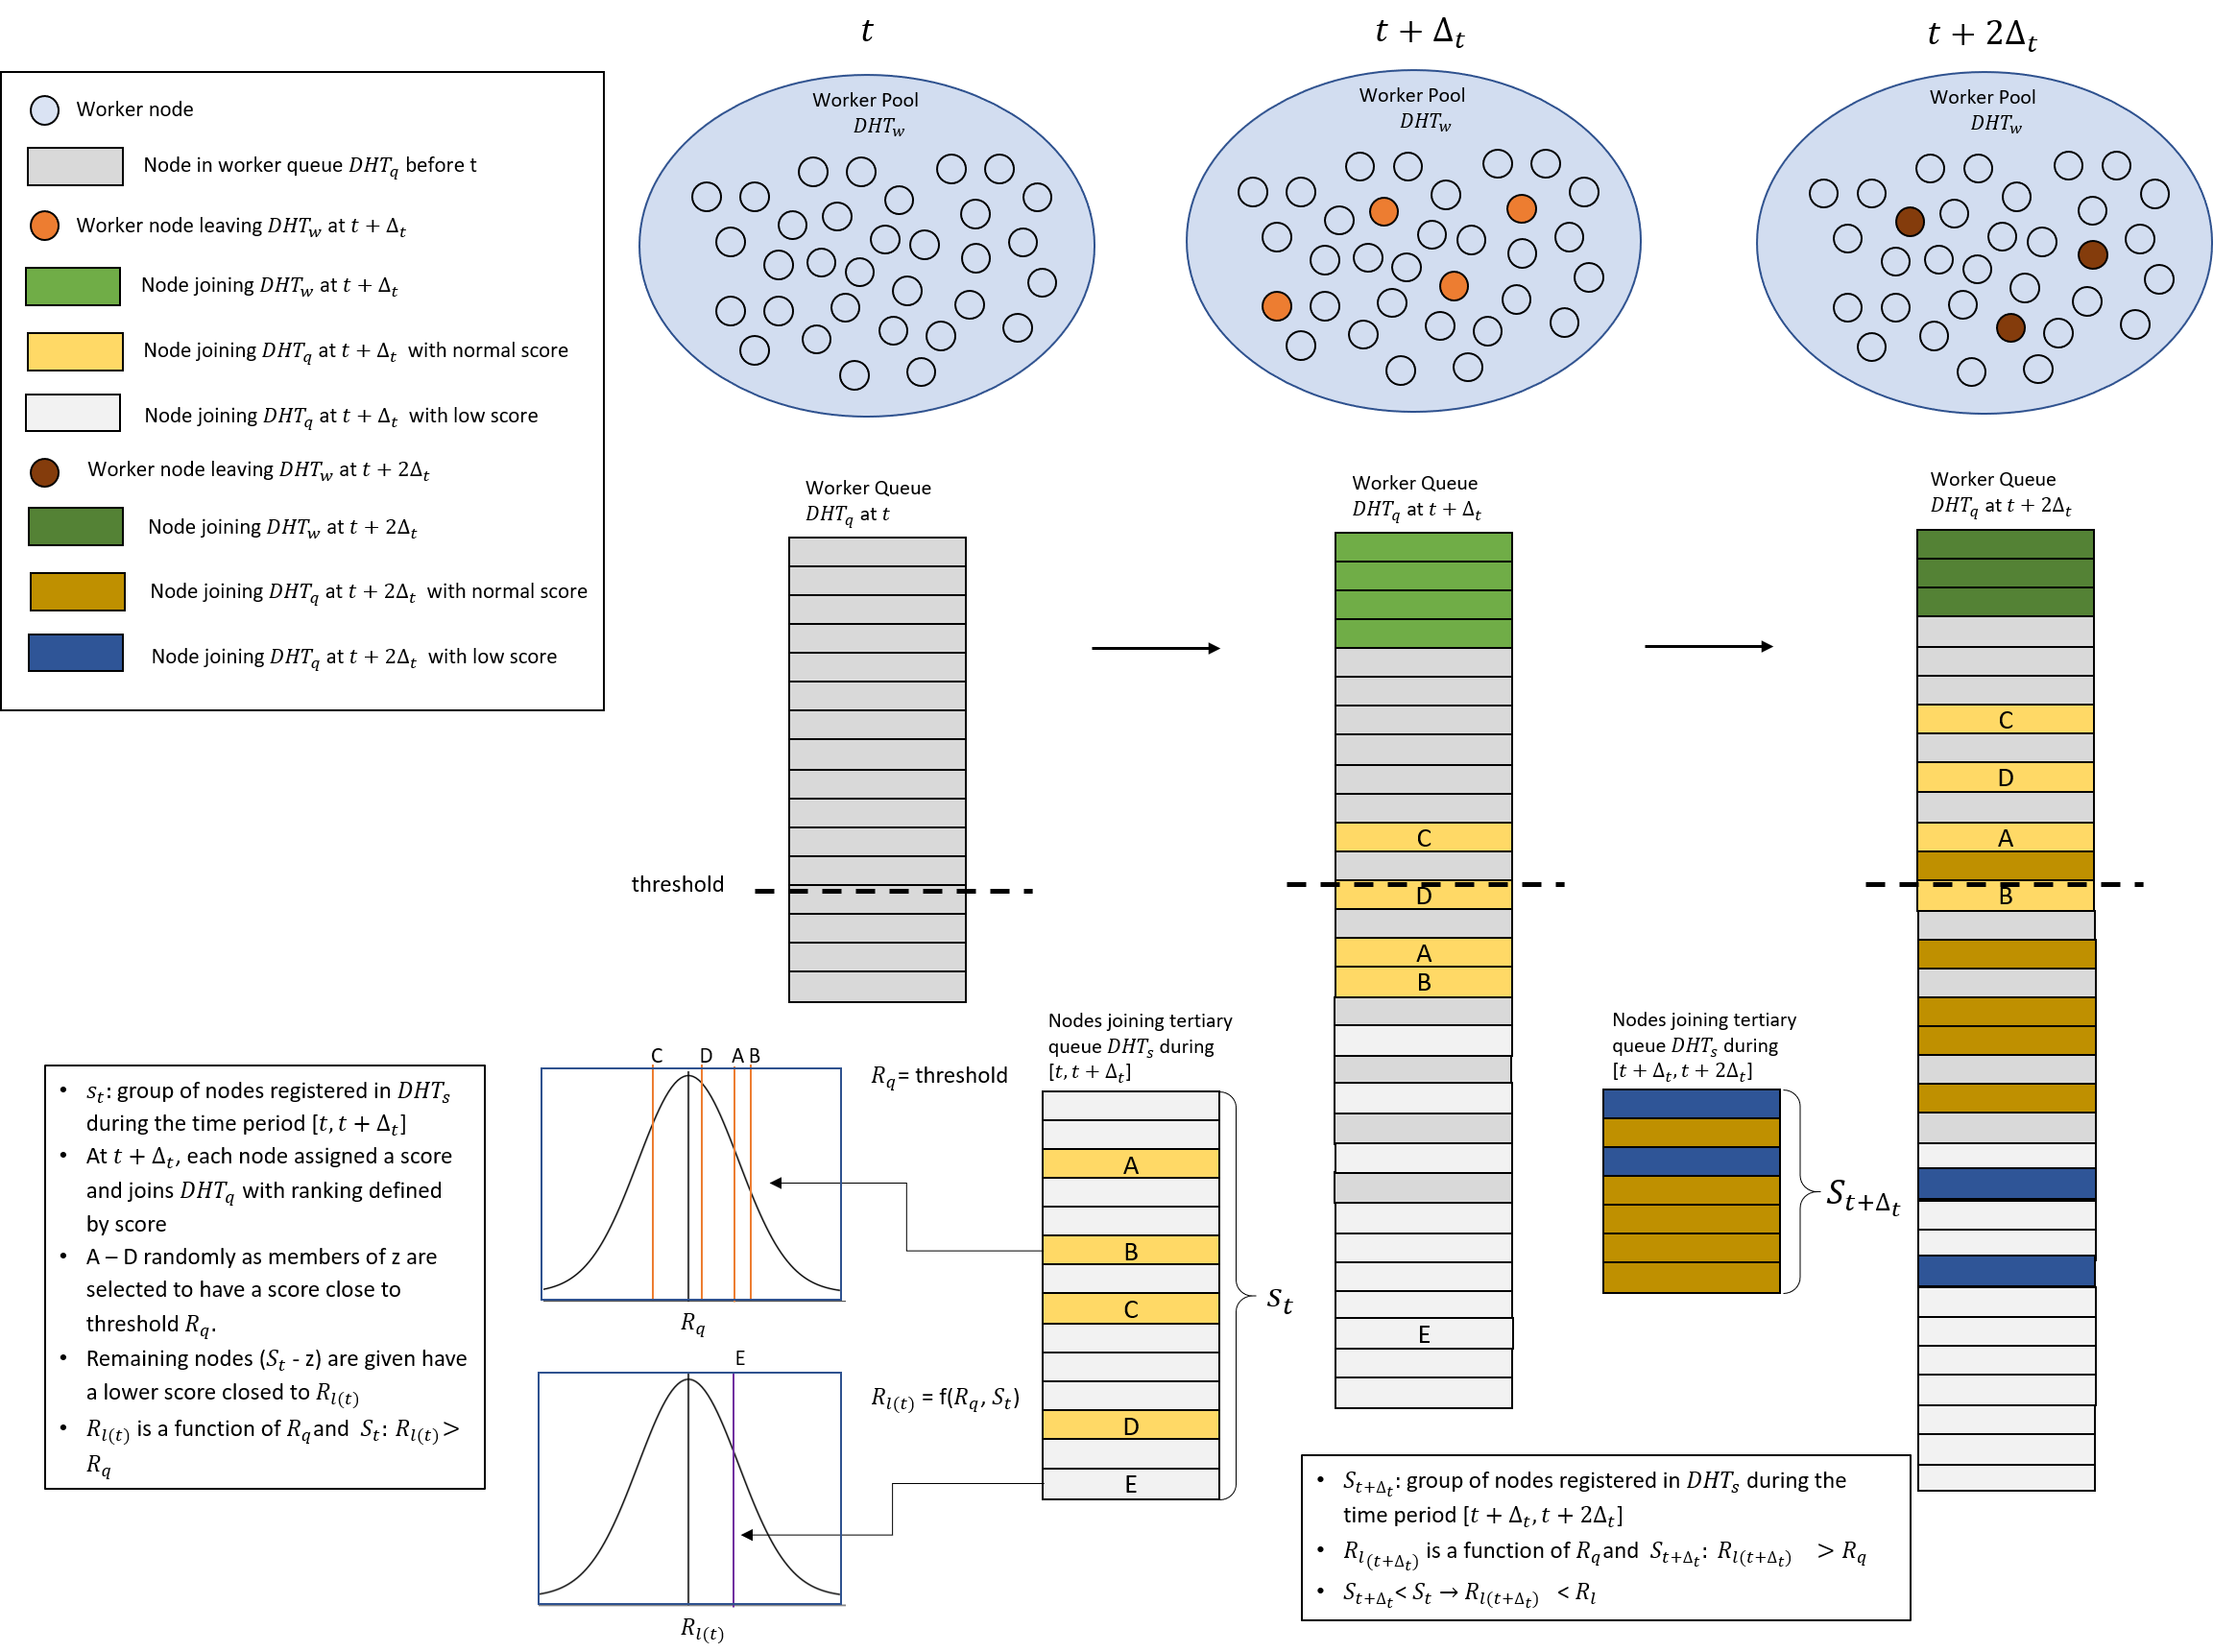
\includegraphics[width=22cm,height=42cm,keepaspectratio]{Figures/Work_Queue_Management}
\caption{\label{fig:NSM}Illustration of the process followed by Catalyst network to add nodes to the work queue.}
\end{figure}
\end{landscape}



%%%%%%%%%%%%%%%%%%%%%%%%%%%%%%%

\chapter{Catalyst Distributed Ledger} \label{Cha:LDA}
The Catalyst database is designed to ensure it can run on low resource devices and fit the different needs of the network users without compromising on data integrity or accessibility. 

\section{Ledger Database Architecture} \label{Sec:LDA}

 Catalyst has a multi-level data architecture, as illustrated in Figure~\ref{fig:db}. 

\begin{figure}[H]
\label{fig:db}
\center{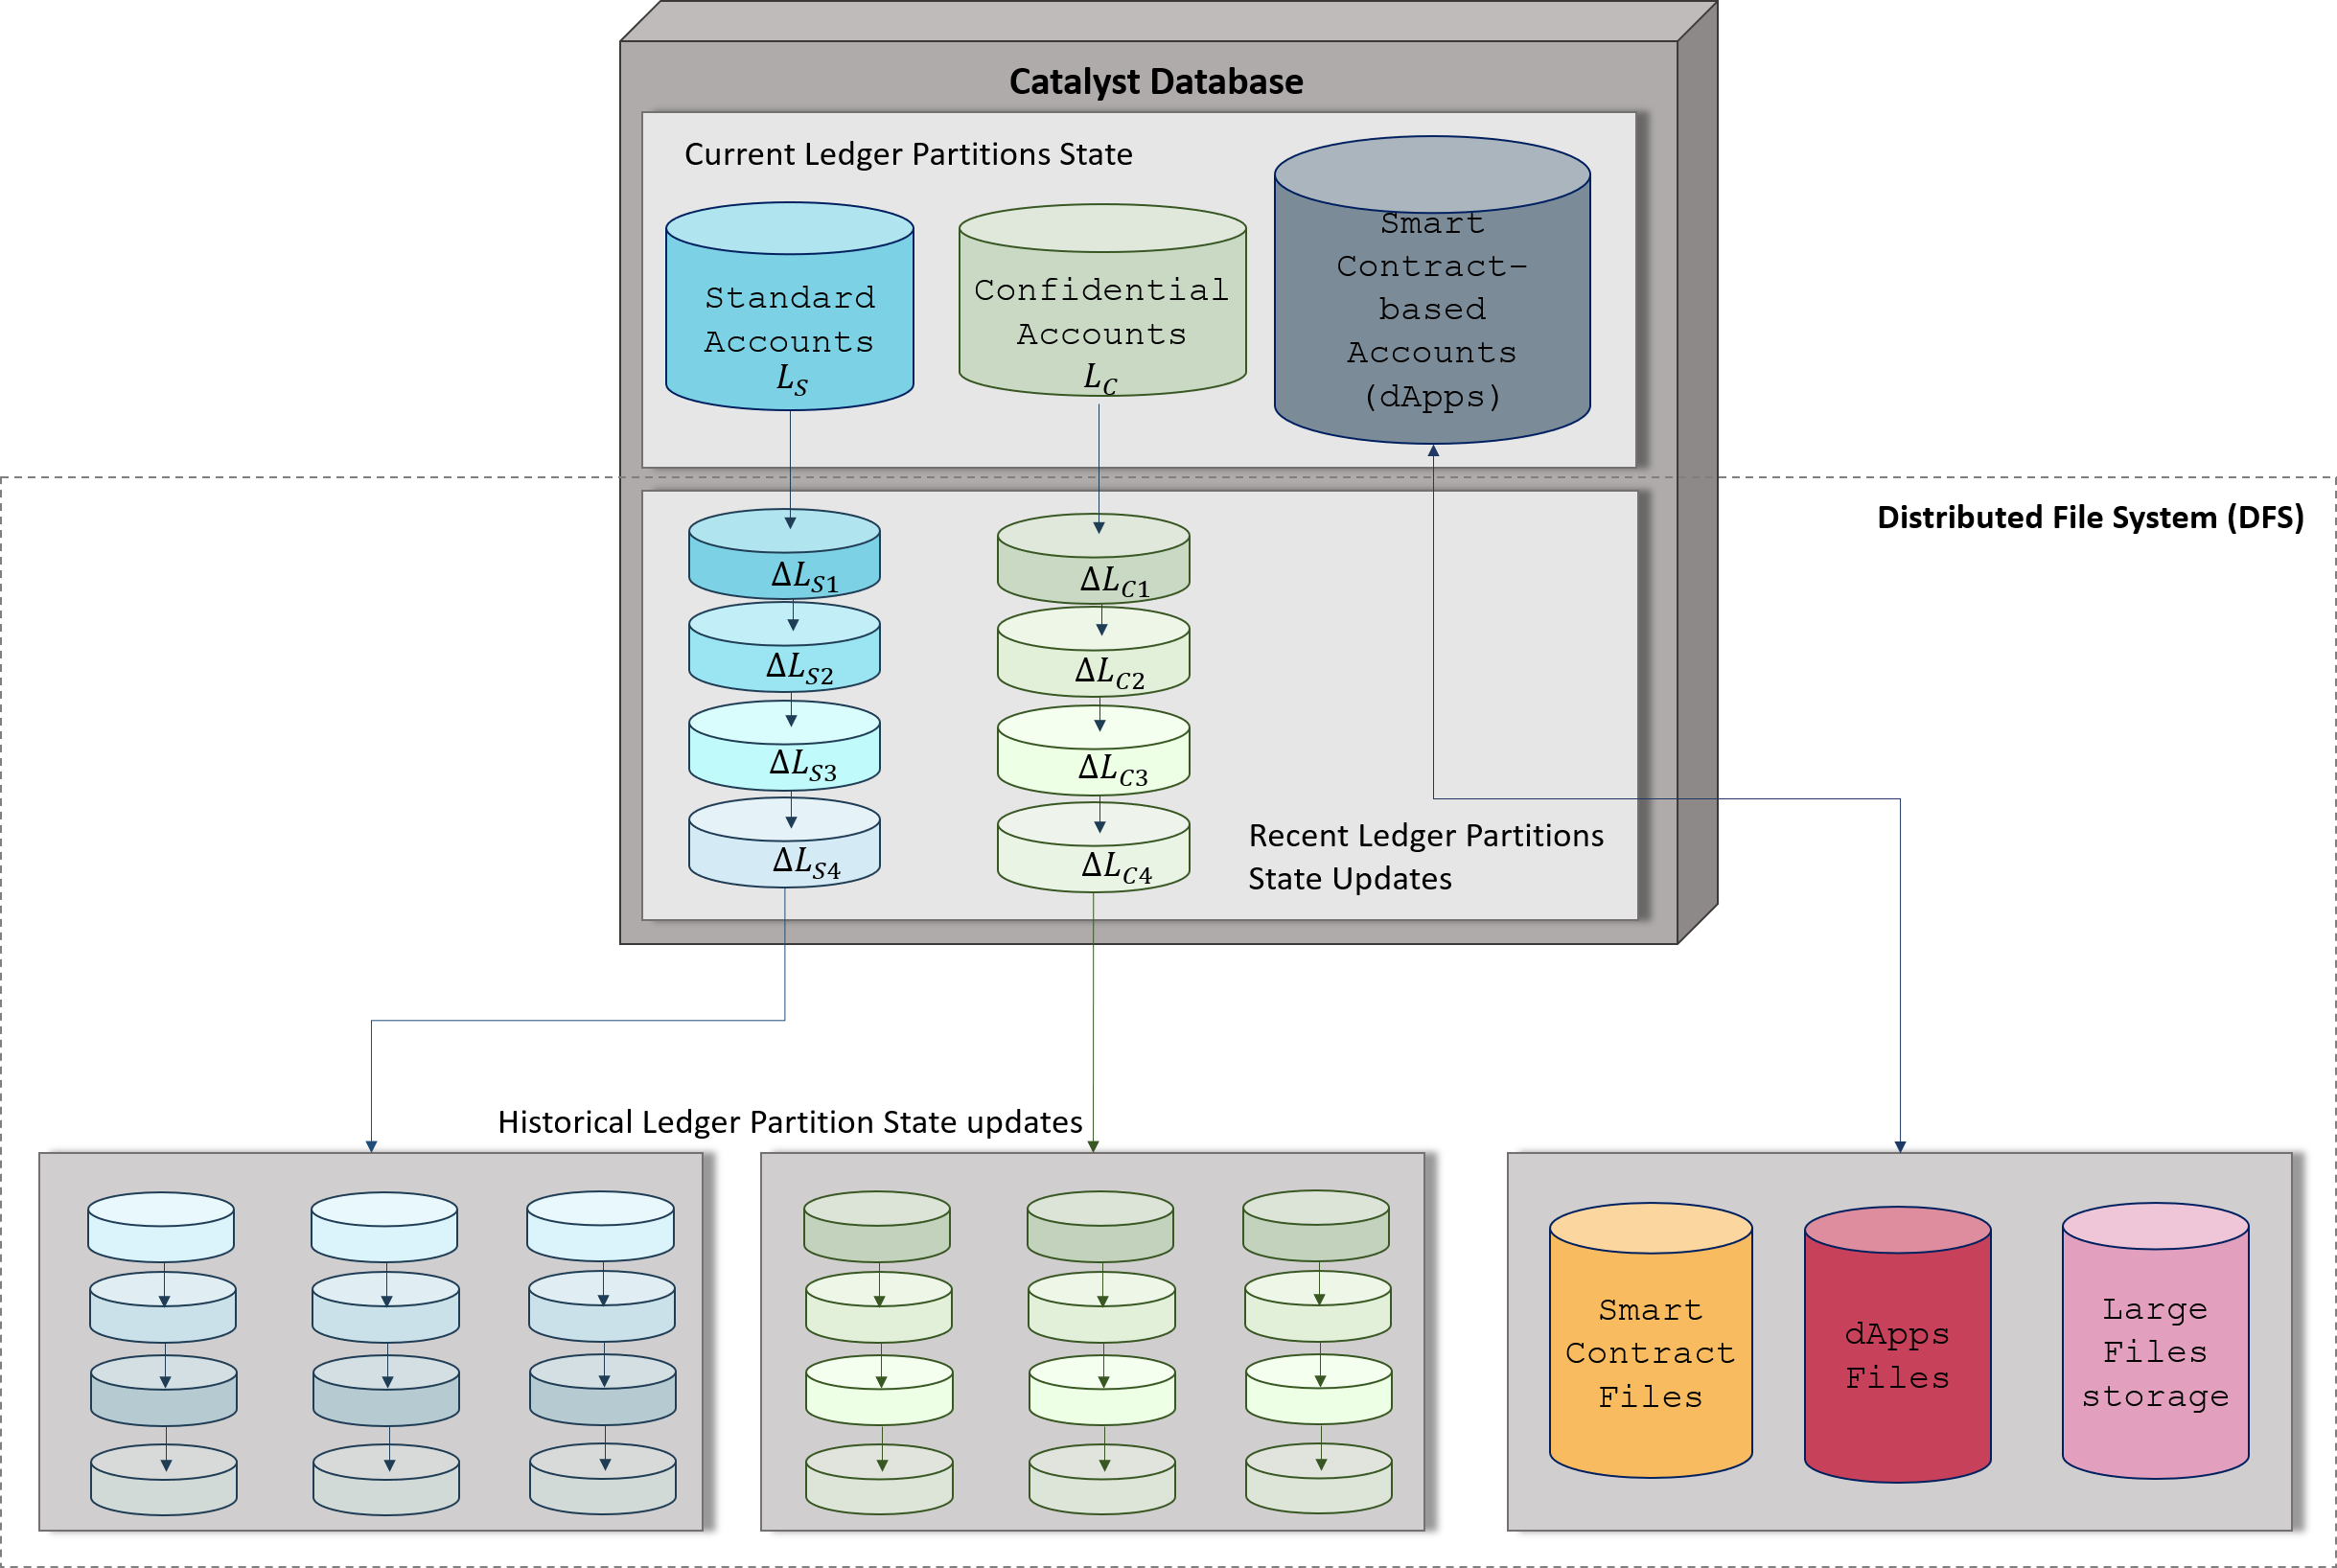
\includegraphics[width=11cm]{Figures/Catalyst_Database}}
\caption{\label{fig:db} Illustration of Catalyst database architecture.}
\end{figure}

At the top level lies the current state of the ledger (CLS), \textit{i.e.} the database containing the current balance of digital accounts recorded on the ledger. The CLS represents a snapshot of the ledger state, at the present time. It is periodically updated. At the end of a ledger cycle, that lasts for a fixed period between 30 seconds and 1 minute, a ledger state update is generated by a pool of nodes selected to manage the ledger database, the producers, and distributed to the network users who can then update their local copy of the ledger state. The process followed by producers to generate a ledger update, \textit{i.e.} the consensus-based protocol, is described in section~\ref{Sec:Dem}.\\

The middle level comprises the recent ledger state updates, that is a set of the last recent ledger state updates accepted by producers and broadcast across the network. Historical data, or old ledger state updates, represent the bottom level. Both middle and bottom levels are maintained by Catalyst Distributed File System (DFS) module. The top and middle levels sits on every node on the network and are thus immediately accessible. On the other hand the bottom level is maintained by some but not necessarily all nodes in the network. Long term data is thus available with a short delay which constitutes a small trade-off for a compact ledger database maintained by every node.\\

Figure~\ref{fig:db} also shows the smart contracts and dApps stored on a database unit separate from the account balances and communicate with DFS for the access, production and storage of files. Technical specificities around smart contracts and dApps are discussed in a paper soon to be released.



\section{Accounts on Catalyst} \label{Sec:AoC}

Different types of accounts are stored on Catalyst ledger. Namely:

\begin{itemize}
\item Non-confidential user-based accounts, with a balance in KAT tokens that is updated via the validation of non-confidential transactions. The account balance is visible to all.
\item Confidential user-based accounts, with a balance in KAT tokens that is updated through the validation of confidential transactions. The account balance is hidden, only known to the account holder(s).
\item Smart contract-based accounts. A smart contract-based account has an associated code that can be triggered by transactions or messages generated by other codes.
\end{itemize}

An account comprises the following components: 

\begin{itemize}
\item An address component: a 20-byte address $A_{i}$, which is derived from a public/private key pair \{$Q_{i},k_{i}$\} (where $Q_i= k_{i}G$, $G$ is an EC generator) using a collision-resistant hash function ($\mathcal{H}$): $A_{i} = \mathcal{H}(Q_{i})$. The last 20 bytes of the hash are used to create the address. A prefix is added to distinguish between the different types of accounts.
\item An amount component: when non-confidential, the amount is a 8-byte number $v_{i} \in \mathbb{Z}_M$. This represents the account $A_{i}$ balance in KAT tokens (with $M$ a threshold on the number of tokens). When confidential, the amount component is a 32-byte Pedersen Commitment~\cite{confidential} $C_{i} = v_{i}H + b_{i}G$ that hides the balance $v_i$ of the account using a blinding factor $b_{i} \in \mathbb{Z}_p$ ($p \gg M$).
\item A data component: reserved to smart contract-based accounts and used to store data (or a reference to data stored on DFS) that amounts to a maximum of 64 bytes. 
\end{itemize}

As such, Catalyst ledger state is naturally split into sub-states, or shards, where each shard stores accounts of a given type. A node on Catalyst network may not maintain a copy of all shards but must remain aware of the possible dependencies among shards\footnote{The section discussing sharding techniques applied to Catalyst is under construction.}.%(see chapter~\ref{Cha:Sha}).\\

\section{Ledger Current State and DFS}\label{Sec:DFS}

The ledger state thus encompasses different sub-states, each of which keep the balance of accounts of a specific type up-to-date. The current state of the ledger state lists the accounts balance at the present time, allowing anyone to access (and comprehend in the case of non-confidential accounts) the available balance in tokens of an account. \\

When users on the network wish to transfer tokens to other users, they issue transactions that are broadcast to the network. The structure of these transactions are discussed in chapter~\ref{Cha:Tra}. The transactions are collected by nodes assigned to the management of the ledger database (as detailed in section~\ref{Sec:PRT}) and used to generate a ledger state update. The production of valid ledger state updates in a trust-less environment in discussed in chapter~\ref{Cha:CM}. The ledger state update is a cryptographically secure structured data object that allow users to update their local copy of the ledger. \\

The ledger state update consists in a summary of the token transfers embedded in the transactions broadcast by the users. Transactions broadcast during a ledger cycle are collected by nodes who then uses these to generate a ledger state update during the next ledger cycle.  In layman's terms, the ledger state update can be viewed as a structured database with a series of row, each row having two components: a public key referring to the address of an account stored on the ledger and an amount (positive or negative) that represents a token transfer.\\ 

Assume for instance that Alice transfers 5 KAT tokens to Bob. The transfer is represented by a transaction with two entries. The ledger state update would include two rows: one with Alice's address and a negative amount $-5~KAT$ and one with Bob's address and a positive amount $5~KAT$ (transaction fees, discussed in section~\ref{Sec:TStru} are ignored here). Once a user receives a valid ledger state update, the former can use the latter to update their local copy of the ledger: Alice account is debited of 5 tokens while Bob's account is credited of 5 tokens. Note that the ledger state update produced for one ledger cycle only includes balance changes of accounts called in the transactions broadcast on the network during the precedent ledger cycle. This allows for a compact ledger state update as there may be many more accounts stored on the ledger that are not used during a ledger cycle.\\

Transactions in the context of DLT refer to data objects created and cryptographically signed by users and propagated as messages on the peer-to-peer network. A transaction typically includes:

\begin{itemize}
\item a set of inputs where each input comprises the details of the account or digital address being debited, the amount being debited and the signature of the account owner, proving the legitimacy or ownership of the tokens as well as the valid balance of the debited account. 
\item a set of outputs where each output comprises the details of the account being credited. Rather than a signature, a locking program is attached to the output, that effectively locks the tokens sent to this output using the public key of the recipient (the user holding the account being credited).
\end{itemize}

A digital signature associated to a transaction input is a mathematical scheme that allows the owner of the associated private key to prove that they have authorised the spending of the funds locked in the output of a transaction stored on the ledger. A valid signature further guarantees the non-repudiation of the message (the sender cannot deny having sent the message) and the message integrity (the latter has not and cannot be tampered with). \\

In the Bitcoin blockchain, valid blocks of transactions get appended to the blockchain in such a way that any block is cryptographically sealed and linked to the previous valid block. A block contains a set of transactions that transfers digital assets from one digital address to another, as well as an extra coinbase transaction that rewards the miner who successfully produced that block with new digital coins. Each transaction input contained in a valid block (except the coinbase transaction input) refers to the output of a transaction stored on a previous block (a.k.a unspent transaction output – UTXO).  It can actually be viewed as the second state of that output. First the output is unspent and locked, stored on valid block. Secondly, the output is used as input in a new transaction and unlocked by the owner of the unlocking key. Eventually an old block in the blockchain will solely contain spent transaction outputs used as inputs in transactions stored in other later blocks. As such the old block becomes obsolete as it no longer holds any spendable tokens. \\

\textcolor{bulg}{The Catalyst ledger operates differently in the sense that it does not have UTXO. The ledger state comprises digital accounts of which the balance changes over time as transactions debiting or crediting these accounts are validated on Catalyst network. Once a ledger state update is used to update the ledger database of accounts, the ledger state update is stored on DFS and can be accessed by any node as it is either locally stored or accessible upon request to special nodes storing historical data (bottom level). User nodes need not access to old ledger state update to be able to transfer tokens from their account stored on Catalyst ledger. They only need  a local copy of the current ledger state. DFS is built upon the IPFS protocol which is not novel. It is nevertheless used to store files as well as historical ledger state updates. This removes the burden on user nodes to maintain the full history of the ledger database while allowing for fast retrieval of files as well as old ledger state updates. DFS is maintained by all nodes on the network. However, DFS is made of a multitude of compartments and each node needn’t hold all compartments.}\\

\textcolor{bulg}{The design of a ledger compartment dedicated to the storage of files and historical ledger state update (DFS) is an approach taken to prevent bloating of the ledger and allow the network to hold services a scale. Indeed, this approach allows Catalyst ledger to remain lean and cryptographically secure. As detailed in chapter~\ref{Cha:Tra}, the removal of UTXO is made possible via a new structure of transaction objects in which any token transfer (wherever spending or receiving tokens) is signed and thus authorised by the relevant participants involved in said transfer.}



%%%%%%%%%%%%%%%%%%%%%%%%%%%%%%%
\chapter{Transactions} \label{Cha:Tra}

Transactions are the integral element to any blockchain or DLT. These are messages broadcast by users on the network that encompass the transfer of tokens and data to and from digital accounts stored on the ledger. Catalyst network strives to offer users a variety of services accessible on the network and as such supports a plurality of transaction types. This includes the choice of opting for hidden or visible accounts via the support of both non-confidential and confidential transactions, thus offering different levels of anonymity to the network users. This section describes how different transaction structures and account types are supported on Catalyst and details the processes behind the generation and verification of transaction signatures. 


\section{Transaction Types} \label{Sec:Typ}

On the Catalyst ledger, a transaction is a message or object used to transfer KAT tokens or data from and to a set of digital accounts. Such a transaction can include different types of transfer depending on the nature of the accounts embedded in said transaction. As mentioned in section~\ref{Sec:AoC}, Catalyst supports the transfer of confidential and non-confidential assets. Catalyst also supports the transfer of assets and data linked to smart contracts and data storage. These different types of transfer are defined by specific transaction components that allow any node on the network to differentiate between the nature of exchanges embedded in different transactions. In this section we give an overview of the transaction structure and the different components considered for each type of token and data exchange.

\section{Transaction Structure} \label{Sec:TStru}

In traditional blockchains (such as Bitcoin) a transaction is composed of a set of inputs and outputs. An input refers to the output of a transaction stored on a valid block of the blockchain, effectively spending that output (also referred as UTXO). In broad terms, an input thus spends tokens, while an output receives some. The output is locked and can later be spent in an input of a future transaction. On the Catalyst ledger, we opt for a new terminology, defining as \textit{transaction entry} a transaction component that spends or receives tokens.\\

A transaction object on Catalyst is made of the following components:

\begin{itemize}
\item A transaction type specifying the type of exchange embedded in the transaction entries (non-confidential or confidential asset transfer, data storage request and retrieve, smart contracts-related token and/or data transfer).      
\item A timestamp corresponding to the point in time the transaction is complete and ready to be broadcast on the network.
\item A set of $n$ transaction entries $\{E_i\}_{i=1,..,n}$. Transaction entries are specific to the nature of the token and data exchange. These are described in \ref{Sec:TEnt}.
\item An aggregated signature $T$ proving ownership of the set of accounts called in the transaction entries.
\item A locking time corresponding to a point in time after which the transaction can be processed by a worker pool.
\item The transaction fees paid by the transaction participants
\item A data field that can contain up to 60 bytes of data transferred in data storage or smart contract-related transactions. 
\end{itemize}

Any valid transaction must contain a type, a timestamp and locking time (the later is set to 0 is there is no waiting period prior to processing a token exchange embedded in the transaction), a list of transaction entries and an associated signature. Any other field can be included to the transaction, depending on the nature of the token exchange. 


\section{Transaction Entries}\label{Sec:TEnt}

Transaction entries are used on the Catalyst ledger to represent the transfer of tokens into or out of the account referenced in the entries. This generally takes the form of debit or credit of an account. We use the term entry to replace the traditional input and output, as on Catalyst there is no differentiation as to how the debit or credit of an account is formed. Whether spending or receiving tokens, a user must sign their transaction entry and a transaction is complete if and only if all transaction entries have been signed.\\

 A transaction entry typically consists of two components: 
 \begin{itemize}
\item A public key, from which the address of an account stored on the ledger is derived.
\item An amount component that can be a number (when the transaction is non-confidential) or a Pedersen commitment (when the transaction is confidential) and represents the number of tokens spent from or transferred to the address associated with the public key.
%\item and a fee component that is a number representing the amount of tokens paid as transaction fees. 
\end{itemize}
On Catalyst, the amount or number of tokens included in a transaction entry can be positive (when receiving) or negative (when spending). This choice allows for a) keeping a simple transaction entry structure (there is no need for an extra field to specify the type of transfer embedded in an entry) and b), in the case of confidential asset transfer, an improved anonymity as an observer will be unable to differentiate between a sender and a recipient in a token transfer. \\

The public key $Q_i$ in a transaction entry $E_i$ is always a 32-byte element from which one address $A_i$ stored on the ledger can be derived. \\

The amount component of an entry however differs depending on the nature of the token exchange:

\begin{itemize}
\item For a non-confidential asset transfer, it is a 8-byte (positive or negative) number $v^t_i$ that represents the number of tokens spent from or transferred to the address $A_i$, communicated in clear text.
\item For a confidential asset transfer, it is made of two elements: 
\begin{itemize}
\item A 32-byte Pedersen commitment $C_{i}^{t}$ that represents the commitment of tokens spent from or transferred to the address $A_i$ 
\item A range proof $\Pi_i(C_{i}')$ (as discussed in section \ref{Sec:ZKP}) that proves that the token balance of $A_i$ remains within an acceptable range of value (typically greater than 0 and smaller than a threshold $M$ of number of tokens) after the transaction has taken place.
\end{itemize}
 The construction of these elements is discussed below. 
\end{itemize}

The balance $v_i$ of the account $A_i$ is initially represented on the ledger by the PC: 
\begin{equation}
C_{i}=(v_i~mod~l_H)H+ (b_i~mod~l_G)G
\end{equation}

Where $b_i$ is a blinding factor chosen by the account holder. Let's assume that the latter wishes to exchange a number $a_i$ of tokens. To obfuscate the amount of tokens transferred in a transaction entry $E_i$, the account holder creates a PC: 
\begin{equation}
C_i^{t} = (v_i^{t}~mod~l_H)H+ (b_i^{t}~mod~l_G)G
\end{equation}

Where $v_i^{t} = a_i$ if receiving the tokens ($a_i > 0$) and $v_i^{t} = l_H+a_i$ if spending the tokens ($a_i<0$). $l_H$ is the order of the subgroup of EC points generated by $H$ and is much greater than $K$, the maximum number of KAT tokens defined in Catalyst system. As a result, it would not be possible to construct a valid range proof for $v_i^{t}$ when $a_i<0$. The account holder can however create a second PC as follows:
\begin{equation} 
C_{i}'=(v_i'~mod~l_H)H+ (b_i'~mod~l_G)G
\end{equation}

Which represents the commitment of the account balance after the transaction has taken place:
\begin{center}
\[
C_{i}' = C_i + C_i^{t}\begin{cases}
               v_i' = v_i + v_i^t\\
               b_i' = b_i + b_i^t
            \end{cases}
\]
\end{center}

If $a_i<0$, $v_i'H = [v_i + (l_H+a_i)mod~l_H]H = [v_i + a_i]H$. It is only possible to generate a valid range proof associated to $C_{i}'$ if $v_i > a_i$. Note that $v_i$ is necessarily smaller than $M$ as the balance of the account would have been determined by a previous transaction entry, itself including a range proof ensuring that $v_i~\in~[0,K)$. As discussed in section~\ref{Sec:ZKP}, a range proof generated using the bulletproof protocol amounts to 672 Bytes. \\

Table~\ref{tab:TrSt} summarises the different components of a transaction and their respective size for the two types of transfer aforementioned. \\

\begin{table}[htbp]
\centering
\begin{tabular}{ | l | l | l | l | }
    \hline    
    \multicolumn{3}{| l | }{\textbf{Transaction message}} & \textbf{Size} \\ \hline \hline
     \multicolumn{3}{| l | }{Transaction Type (account type \& asset class) } & 1 Byte \\ \hline


       \multirow{ 4}{*}{Entries ($n>1$)} & \multirow{ 2}{*}{non-confidential entry} & 32-byte public key &  \multirow{ 2}{*}{$n \cdot 40$ Bytes} \\
     \cline{3-3}
    	& & 8-byte amount &\\  
     \cline{2-4}

                   &   \multirow{ 2}{*}{or confidential entry} & 32-byte public key &  \multirow{ 2}{*}{$n \cdot 736$ Bytes} \\
     \cline{3-3}
   	&   & 32-byte PC &\\ 
     \cline{3-3}
	& & 672-byte range proof &\\ \hline

 \multicolumn{3}{| l | }{Transaction fees} & 8 Bytes \\ \hline 
 \multicolumn{3}{| l | }{Locking Time} & 4 Bytes \\ \hline
 \multicolumn{3}{| l | }{Aggregated Signature} & 64 Bytes\\ \hline
 \multicolumn{3}{| l | }{Timestamp} & 4 Bytes \\ \hline
    \end{tabular} \\ 
\caption{Structure of confidential and non-confidential transactions on Catalyst and size per transaction component.}
\label{tab:TrSt}
\end{table}

Each entry in a transaction needs to be signed to authorise the transfer of tokens from or to the address included in said entry. This can be achieved through the use of an aggregated signature scheme as described in section \ref{Sec:Sig}. \\

Another type of transaction entry is considered on Catalyst, that is a stand-alone entry. It is not included in a transaction but is added to the ledger state update generated by the producers during the ledger cycle and includes the reward allocated to a specific producer for its contribution in producing a valid update of the ledger state. Such entry, called \textit{ledger compensation entry} (or simply compensation entry), is very similar to a non-confidential entry. It includes an 8-byte amount, that is however always positive, and a 32-byte public key from which the address of an account stored on the ledger is derived. However, unlike transaction entry, a compensation entry need not be signed to authorise the transfer of tokens to the account address specified in said entry. 



\section{Transaction Signature}\label{Sec:Sig}

On the Catalyst ledger, all the transaction entries are signed to authorise the transfer of tokens which means that all the participants in the transaction need to sign their respective entry for a transaction to be considered complete. When signing an entry $E_i$ a participant needs to prove ownership of the account $A_i$ referred in said transaction entry. Said otherwise, the user needs to prove knowledge of the private key $k_i$ paired the public key $Q_i$ from which the account address $A_i$ is derived. A verifier can verify the validity of the signature given the public key $Q_i$ specified in an entry $E_i$.\\

Signatures for transactions on the Catalyst network are formed in a highly similar way regardless of whether the asset transfer embedded in said transaction is confidential or non-confidential. The signature scheme describes in this section therefore applies to both transaction types unless explicitly stated. \\

In blockchains such as Bitcoin and Ethereum, transaction inputs are signed using ECDSA scheme, where the public key is recovered from the signature and used to retrieve the account or UTXO address, thus ensuring that the rightful owner of the tokens is authorised to spend these. The use of a second temporary, often called ephemeral public/private key pair in the signature adds a layer of protection against malicious attempt to retrieve the private key of a user when signing multiple transactions spending tokens from the same address.\\
 
 Public key recovery is however incompatible with batch validation, \textit{i.e.} it is not possible to recover a set of public keys from an aggregated signature on multiple transaction inputs. As a result the choice of ECDSA-based scheme for Catalyst transaction would not be optimal as a transaction contain a minimum of two entries. A Schnorr-based signature scheme is preferred to enable user to jointly produce a signature using their private keys. A solution recently proposed by Y. Seurin \textit{et al}~\cite{schnorr} also accounts for protection against key-rogue attacks, preventing key malleability to create validate signatures on transaction without knowing the users' private key. We propose a Schnorr-based signature scheme inspired from this recently published work. \\

We define the transaction core message $m$ as a set of $n$ entries $\{E_i\}_{i=1,..,n}$ and additional information $X$ mentioned in the previous section (see table~\ref{tab:TrSt}), excluding the transaction timestamp:
\begin{center}
$m = \{E_i\}_{i=1,..,n} + X$ 
\end{center}

The participant $U_i$ responsible for $E_i$ (holder of the account $A_i$) creates the following challenge:
\begin{equation} 
e_i = \mathcal{H}(m \mid\mid \tilde{Q})\mathcal{H}(L \mid Q_i)
\end{equation} 

Where:

\begin{itemize}
	\item$\mathcal{H}$ is a hashing function
	\item$m$ is the transaction core message 
	\item$\mid\mid$ denotes the concatenation between strings
	\item$\tilde{Q}$ is the aggregated public key such that:
\begin{center}
$\tilde{Q}=\mathcal{H}(L \mid\mid Q_1)\cdot Q_1 + .. + \mathcal{H}(L \mid\mid Q_n)\cdot Q_n$
\end{center}
	\item$L$ is the hash of all the public keys used in the transaction expressed as $L=\mathcal{H}(Q_1~||~..~||~Q_n)$
\end{itemize}

$U_i$ then creates the following partial signature:

\begin{equation} 
s_{i} = r_i + e_i\cdot k_i
\end{equation}

Where $r_i$ is a pseudo-random number chosen by $U_i$ and kept secret.\\

 Recall that each entry $E_i$ in a confidential transaction includes a PC obfuscating the amount $v_i^{t}$ defined by: $C_i^{t} = v_i ^{t} H + b_i^{t} G$. For confidential transaction we define $r_i = b_i^t + d_i$ where $d_i$ is a pseudo-random number chosen by $U_i$ and kept secret.\\

The partial signature ($s_i$, $R_i$) with $R_i = r_iG$ is forwarded to the other transaction participants. Each participant in the transaction $U_k$ ($k\neq i$) can compute:

\begin{equation} 
R_i' = s_{i}\cdot G - e_i\cdot Q_i
\end{equation}

where $Q_i = k_i\cdot G$ and verify that $R_i' = R_i$, proving the validity of the partial signature. \\

The last participant to receive the full set of partial signatures builds the transaction signature.\\

 The transaction signature of non-confidential transaction is composed of the pair:
\begin{equation} 
T= (\underbrace{s_{1}+..+s_{n}}_{s}, \underbrace{R_{1}+..+R_{n}}_{R})
\end{equation}

At the verification phase, a producer can check that the total signature is as follows:
\begin{enumerate}
\item Compute the list of $n$ challenges $\{e_i'\}_{i=1,..,n}$ given the public keys embedded in the transaction entries $\{E_i\}_{i=1,..,n}$ included in $m$
\item Compute the quantity $R' = s \cdot G - \sum_{i=1}^{n}e_i'Q_i$
\item Verify that $R'=R$
\end{enumerate}

If so, the signature $T = (s,R)$ is valid. The signature is composed of a 32-byte integer and a 32-byte EC point, leading to a compact 64-byte signature for the entire transaction. \\

The transaction signature of confidential transaction is defined differently although its structure is the same as that of non-confidential transaction . Using the public keys $\{D_i = d_iG\}_{i=1,..,n}$, it is composed of the pair:
\begin{equation} 
T= (\underbrace{s_{1}+..+s_{n}}_{s}, \underbrace{D_{1}+..+D_{n}}_{D})
\end{equation}

The verifier can compute:
\begin{center}
$R' = \sum_{i=1}^{n}C_i^t + v^fH + D$
\end{center}

If $R' = s \cdot G - \sum_{i=1}^{n}e_i'Q_i$, the signature $T = (s,D)$ is valid. The validity of $T$ proves a verifier that the sum of the commitments in the transaction entries results in a commitment to 0 after adding the transaction fees paid by the different participant, thus ensuring that no tokens are created or lost in the transaction. \\

Once the transaction signature is valid, the participant can append it to the transaction. The transaction timestamp is defined as the time when the transaction is completed by said participant and ready for broadcast across the network. 



\section{Transaction Validity} \label{Sec:Val}

Nodes in the network receive and forward transactions to their peers. In order to prevent spamming attack over the network,  nodes only forward transactions that are considered valid against a validity check list. Before forwarding it to its peers, a peer verifies the transaction against the following list of criteria:
 
\begin{itemize}
\item The transaction syntax (aforementioned in \ref{Sec:TStru}) and data structure must be correct.
\item The transaction size in bytes is greater than or equal to 160 Bytes (defined by the parameter MIN\_STD\_SIZE for non-confidential transaction) or 800 Bytes (defined by the parameter MIN\_CON\_SIZE for confidential transaction).
\item The transaction size in bytes is less than 1 Mbyte (defined by the parameter MAX\_STD\_SIZE or MAX\_CON\_SIZE depending on the transaction type).
\item The transaction list of entries must have at least two elements, each element must have a correct syntax. 

For non-confidential transaction $E_i$ must have a total size of 48-byte and 3 components:
\begin{itemize}
\item A public key $Q_i$ with a corresponding account address $A_i$ stored on the ledger where the account have a visible balance (8-byte field).
\item An amount $v_i^t$ that once added to the balance $v_i$ of the account mapped with the public key leaves the account balance positive ($v_i+v_i^t > 0$)
\end{itemize}
For confidential transaction $E_i$ must have a total size of 742-byte and 4 components:

\begin{itemize}
\item A public key $Q_i$ with a corresponding account address $A_i$ stored on the ledger where the account has an hidden balance (32-byte field).   
\item A 32-byte PC $C_i^t$ 
\item A 672-byte range proof must validate against a new PC built out of the sum of $C_i^t$ and the account balance $C_i$. 
\end{itemize}

\item The transaction fee amount $v^f$ is greater than a (positive) minimum fee values MIN\_TX\_FEE
\item The relation $\sum_{i=1}^{n}v^t_i - v^f = 0$ must be verified for non-confidential transaction.
\item The transaction signature must validate against the public key built out of the public keys stored in the transaction entries 
\end{itemize}

The verification of the range proofs in the transaction is costly in computer resources, and is therefore only performed by the producers. 

%%%%%%%%%%%%%%%%%%%%%%%%%%%%%%%


\chapter{Consensus Mechanism} \label{Cha:CM}


Proof-of-work (PoW) and derivate algorithms are commonly used to manage blockchain and distributed ledger in a distributed manner. Consensus-based protocols based on such algorithms rely on a plurality of nodes, called miners, competing to generate at fairly regular interval of time a valid block of transactions to append to the blockchain. Part of the competition consists in solving a cryptographic puzzle that ensures the validity of the content of a block. \\

However, this competition amongst nodes wastes a tremendous amount of energy as all miner nodes expend computational power to solve the same problem, yet only the work performed by one node is used to update the blockchain. The energy consumption per year for Ethereum and Bitcoin combined is 66.6 TWh per year which is comparable to yearly energy consumption of Switzerland (61.6 TWh per year) \cite{electric}\footnote{This energy consumption allows approximately 445 million transactions for Bitcoin and Ethereum combined per year \cite{BitTxpD}\cite{EthTxpD}, compared to Switzerland where 820 million debit card transactions are processed per year \cite{swis} for an estimated energy consumption of 0.001358 TWh.}. It is clear that this is not sustainable or environmentally friendly. Moreover, as the difficulty associated with the cryptographic puzzle increases over time, miners are forced to invest in more computer resources to have a chance of earning miner rewards. Such consensus protocols have a clear negative environmental impact and indicate counteractive economic implications with high risk of mining centralisation. \\

This chapter presents a new consensus-based protocol that can be applied to a peer-to-peer network in order to manage a distributed ledger in a fair and secure manner without wasting unnecessary amount of energy. 


\section{Background}\label{Sec:Cbg}

\subsection{Motivation}
The consensus algorithm designed by the engineers and researchers at Atlas City rests on the principle that every node participating in the network can contribute to the ledger state update and should be rewarded accordingly. Indeed, the consensus mechanism was conceived based on the observations that: 
\begin{itemize}
\item In reality, not every node needs to validate every transaction for a network to be secure and a ledger fully decentralised. 
\item Collectively across a network of nodes there is significant distributed computer resources to securely maintain a ledger. Network performance should as a result improve as the network scales up.
\end{itemize}

The PoW algorithm was introduced to solve the General Byzantine Problem among participants in the peer-to-peer network, allowing them to reach consensus without trusting one another~\cite{BFT}. In the PoW algorithm or any derivatives, mining nodes collect and validate all transactions broadcast to the network and form a block with these new transactions. The miners compete to solve a computationally hard problem, the solution of which is used to prove that a block is valid and can therefore be appended to the blockchain. The level of difficulty attached to the cryptographic problem solved by the miners is set by the network to ensure that blocks are produced on a regular time interval (roughly 10 minutes in the case of Bitcoin, and approximatively 17s for Ethereum). Under this scenario, one mining node is rewarded for producing the correct next block of the blockchain (which in the analogy of Catalyst corresponds to the last valid ledger state update). Although the solution to the cryptographic puzzle is hard to find, it is very easy to verify which allow for a fast and secure update of the blockchain.  \\

While this approach provides a secure way to maintain a distributed ledger, it leads to a tremendous amount of wasted computational and electrical energy with high risk of mining centralisation. In the example of Bitcoin, the early blocks were mined by individuals with modest computer resource. 

\begin{figure}[H]
\center{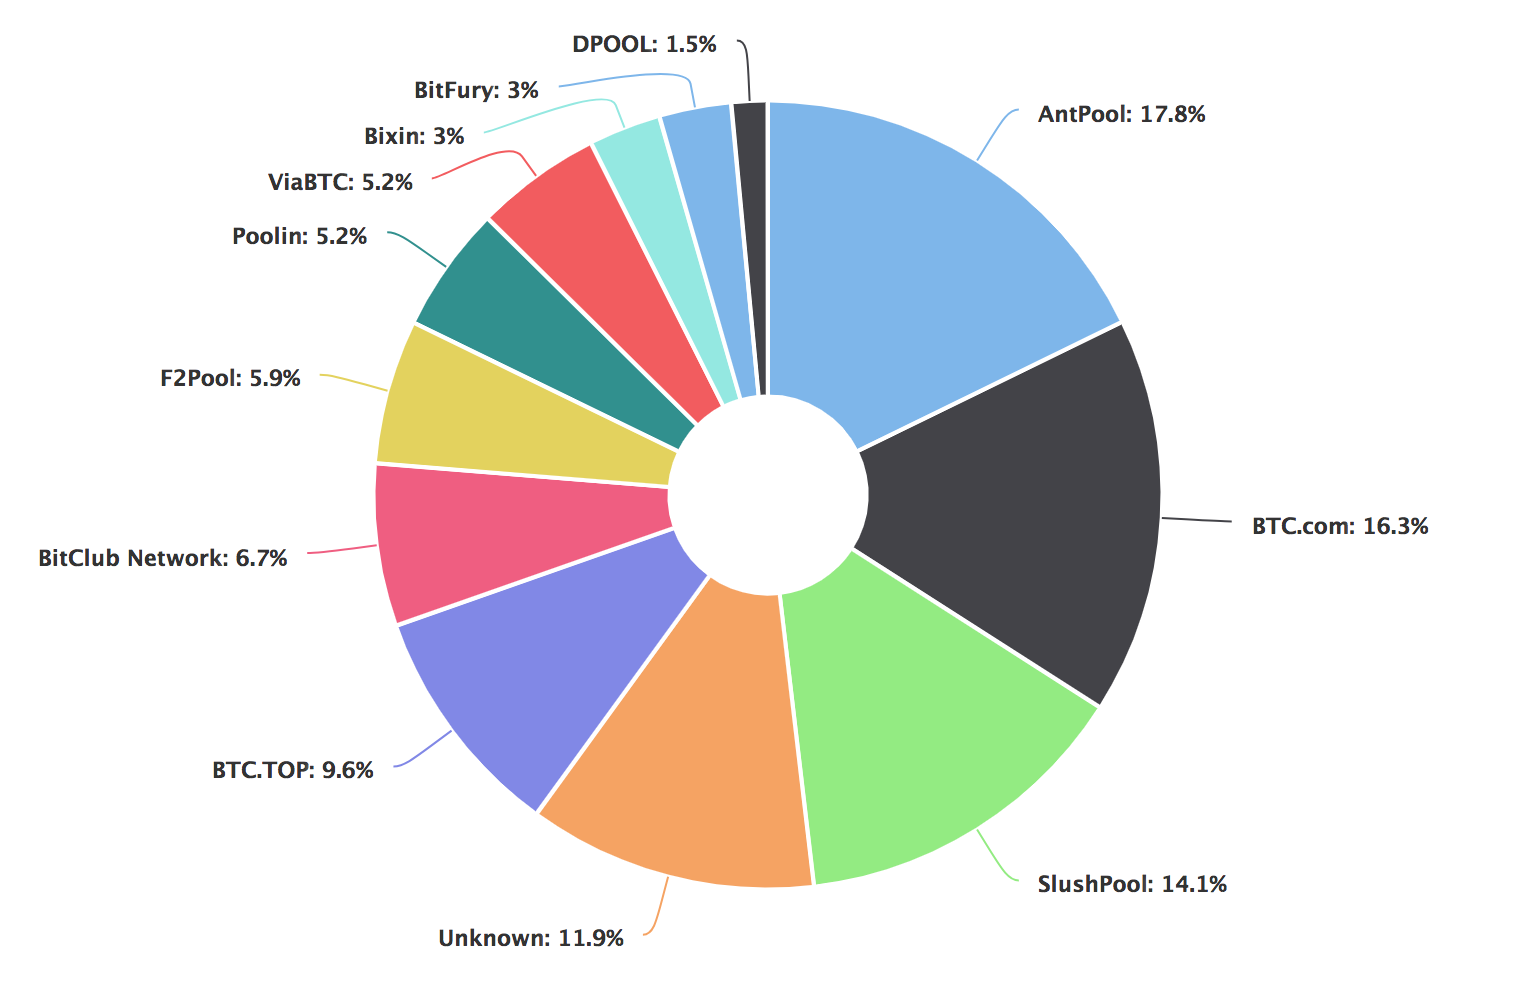
\includegraphics[width=11cm]{Figures/BTC_mining_pools_2018-10-30}}
\caption{\label{fig:pools} Distribution of the Bitcoin hashrate power over a 24h period, as the 30 of October 2018\cite{bc24}}
\end{figure}

As illustrated in Figure~\ref{fig:pools}, the situation is rather different nowadays. Few miners work independently (represented as the “unknown” 11.9\%) while the remaining join mining pools such as Slush Pool (which was the first mining pool created for Bitcoin mining) to share their computer resources and the collected rewards, usually against the payment of a fee (2\% of the mining reward with Slush Pool). Some mining pools are private pool, such as BTC.top. It also worth noting that around 80\% of the mining pools are located in China~\cite{poolcent} where the electricity is considerably cheaper than in other parts of the world.   \\

A popular alternative to the PoW algorithm currently considered by several blockchain projects is the Proof-of-Stake algorithm (PoS). This approach addresses the footprint concerns from the former by assigning the task of producing the next valid bock to a subset of miners. The miner nodes can be selected randomly or based on criteria such as the miner’s wealth (stake). The main concern with a PoS-based consensus mechanism remains the risk for centralisation of wealth and subsequently the network management, with the mining work inevitably distributed to a few wealthy nodes~\cite{PoSr}.\\

\textbf{\textit{Unity is strength}}\\
Catalyst consensus mechanism is not based on a competitive process. Instead, the nodes in the network collaborate to collectively build the correct update of the ledger state. The algorithm used by nodes to produce a valid ledger state update does not require the execution of computationally expensive tasks, allowing nodes with limited resources to contribute. At the end of a ledger cycle, new tokens are injected into the system and all the nodes that contributed to producing the correct ledger state update receive a share of that reward.

\subsection{Naming Convention}

Nodes who contribute to maintaining the ledger state are called producers, rather than miners. Indeed, producers do not solve a computationally hard problem, but instead validate the transactions broadcast to the network and use these to collaboratively build (produce) a ledger state update. \\

In this chapter we assume that the ledger is composed of one single shard comprising a fixed set of accounts. The implementation of sharding techniques are discussed in chapter currently under construction.
%~\ref{Sec:Sca}. 
We therefore consider one single worker pool and one subset of producer nodes selected per ledger cycle. \\

A ledger cycle $\mathcal{C}_n$ starts at time $t = t_{n,0}$ and lasts for a period of time $\Delta t_{cycle}$, therefore ending at $t = t_{n,0}+ \Delta t_{cycle}$. $P$ producers $\{P_j\}_{j\in P}$ are selected to build the ledger state update during the ledger cycle $\mathcal{C}_n$. Each producer $P_j$ can be identified by its peers as well as the rest of the network via its unique identifier $Id_j$ (see section ~\ref{Sec:PIP}).\\

During $\mathcal{C}_n$ the $P$ producers collaborate to create a ledger state update $\Delta L_{n}$ based on the set of $m_{n-1}$ transactions broadcast on the network during the previous ledger cycle $\mathcal{C}_{n-1}$. To limit discrepancies in the set of transactions collected by the different producers and processed during $\mathcal{C}_n$ a small time window $\Delta t_{freeze}$ is considered. The $m_{n-1}$ transactions $\{Tx_j\}_{j=1,..,m_{n-1}}$ are actually collected during the period of time [$t_{n-1,0} - \Delta t_{freeze}, t_{n,0}$] ($t_{n-1,0} = t_{n,0} - \Delta t_{cycle}$) and must have a timestamp comprised between $t_{n-1,0} - \Delta t_{freeze}$ and $t_{n,0} - \Delta t_{freeze}$.\\

Each producer compiles a ledger state update and interacts with its peers to vote on the most popular ledger state update produced by the set of producers. Each producer is thus tasked with two responsibilities: compiling a local ledger state update and voting on the correct (most popular) ledger state update. Each task entitles the producer to receive part of the reward allocated to producers for maintaining the ledger state. The amount of reward individually collected depends on the quality of work performed by a producer. During a ledger cycle $\mathcal{C}_n$, two lists of producer identifiers are created, $\mathcal{L}_n(prod)$ and $\mathcal{L}_n(vote)$. The first one lists the identifiers of producers who correctly built the ledger state update while the second one lists the identifiers of producers who correctly voted on the correct ledger state update built by the producers included in the first list.\\


Throughout the different phases of the ledger cycle, the producers exchange quantities that are hashes, notably of ledger state updates, (using the $Blake-2b$ hashing function) to which they append their identifiers. The exchange of hashes allows for fast and efficient communication rounds amongst the peers as these are smaller pieces of data than the actual ledger state updates. \\

The process followed by producer nodes during a ledger cycle is described in phases. The first three phases consist in producing the correct ledger state update before its broadcast to the entire network. During each phase, a producer $P_i$ generates a quantity $\alpha_i$ and broadcasts it to the network, while collecting the $\alpha_j$ quantities generated by the producers $\{P_j\}_{j\in P/i}$. The final phase ensures the ledger state is updated  across the network. 


%Namely, a computation phase during which the producers locally generate a ledger state update, a voting phase during which the producers reach consensus on the correct set of changes to distribute to the rest of the network and a synchronisation phase during which the correct update including the reward to producers is distributed and the ledger state  is updated by all nodes in the network. 


\section{Democratic Consensus}\label{Sec:Dem}

Section~\ref{Sec:Reg} describes how user nodes register to become worker nodes and can be selected from the worker pool to become a producer for a ledger cycle. This section describes the work performed by producer nodes in order to maintain the ledger state. The work performed by producers in order to generate a ledger state update $\Delta L_n$ for the ledger cycle $\mathcal{C}_n$ starts at $t=t_{n,0}$ and last for a period of time $\Delta t_{cycle}$. At the end of the ledger cycle, nodes in the network use $\Delta L_n$ to update their local copy of the ledger state. This section describes the different phases of a ledger cycle. 

%%%%%%%%%%%%%%%%%%%%%%%%%%%%%%%%%%%%%

\subsection{Construction Phase}
\label{subsec:comp}

During the first phase (\textit{a.k.a} construction phase) of the ledger cycle $\mathcal{C}_n$, a producer $P_j~\forall j \in P$ creates a local ledger state update and exchanges it with its peers.\\

The first phase starts at $t = t_p = t_{n,0}$ and lasts for a period of time $\Delta t_{p}$, therefore ending at $t_p+\Delta t_{p}$.

\subsubsection{Local ledger state update generation and broadcast}

At $t = t_p$, the producer $P_j$ flushes its mempool from the $m_{n-1}$ transactions $\{Tx_i\}_{i=1,..,m_{n-1}}$ collected during the period of time [$t_{n-1,0} - \Delta t_{freeze}, t_{n,0}$] and uses these transactions to create a local ledger state update $\Delta L_{n,j}$. The production of $\Delta L_{n,j}$ lasts for a period of time [$t_p, t_p+ \Delta t_{p0}$] ($\Delta t_{c0} < \Delta t_{p}$). The producer uses a salt $s$, defined using a pseudo-random number generator that takes for seed the hash of the previous valid ledger state update $\Delta L_{n-1}$. The producer also creates a new hash tree $d_n$, to store the aggregated signature embedded in each of the $m_{n-1}$ transactions. $P_j$ then follows a series of steps: 

\begin{enumerate}
\item For each transaction $Tx_i~\forall i\in [1,m_{n-1}]$, $P_j$ verifies that the transaction is valid (see section~\ref{Sec:Val}) and if so, extracts the $n_i$ transaction entries (described in section \ref{Sec:TEnt}) $\{E_\alpha\}_{\alpha=1,...,n_i}$, included in $Tx_i$. The producer also extracts the transaction signature and adds it to the hash tree $d_n$. Note that the transactions signature in $d_n$ are sorted in alphabetic order, as to ensure that two same sets of transaction signature result in the same hash tree.

\item For each transaction entry $E_\alpha$, $P_j$ creates a corresponding hash variable: 

\begin{center}
$O_\alpha = \mathcal{H}[E_\alpha~||~s]$
\end{center}

Each pair ($E_\alpha,O_\alpha$) is added to a list $L^s_E$. Steps (1) and (2) are repeated until all transactions have been processed.

\item	$P_j$ then creates a new list $L^f_E$ using the $M=\sum_{i=1}^{m_{n-1}}n_i$ transaction entries listed in $L^s_E$ (assuming all transactions are valid) such that the transaction entries in $L^f_E = \{E_\beta\}_{\beta=1,...,M}$ are sorted following a lexicographical order based on their associated hash variable: $O_1 < O_2 < ... < O_\beta < ... < O_M$. This approach blurs the links between the token flows embedded in the transactions for a better anonymity of the users involved in said transactions.

\item $P_j$ also extracts the transaction fees $v^{f}_i$ paid in each transaction $Tx_i$ and creates the following sum:
\begin{center}
$x_f = \sum_{i=1}^{m_{n-1}} v^{f}_i$
\end{center}

\item $P_j$ computes the local ledger state update as the transactions entries list $L^f_E$ concatenated with the hash tree of the transactions signature $d_n$: 
\begin{center}
$\Delta L_{n,j} = L^f_E~||~d_n $ %+ x_f
\end{center}

The producer then computes a second quantity that represents its individual contribution:
\begin{equation}
\label{eq:hj}
\fbox{$h_j = h_{\Delta j}~||~Id_j$}
\end{equation}
with $h_{\Delta j}$ referred as the producer \textit{local hash}:
\begin{center}
$h_{\Delta j} = \mathcal{H}(\Delta L_{n,j})$ 
\end{center}
$h_j$ includes the producer unique identifier $Id_j$ (described in section \ref{Sec:PIP}), used to verify that $P_j$ is a producer node selected for the ledger cycle and later evaluate the quality of work performed by $P_j$. 

\begin{figure}[H]
\label{fig:LLSU}
\center{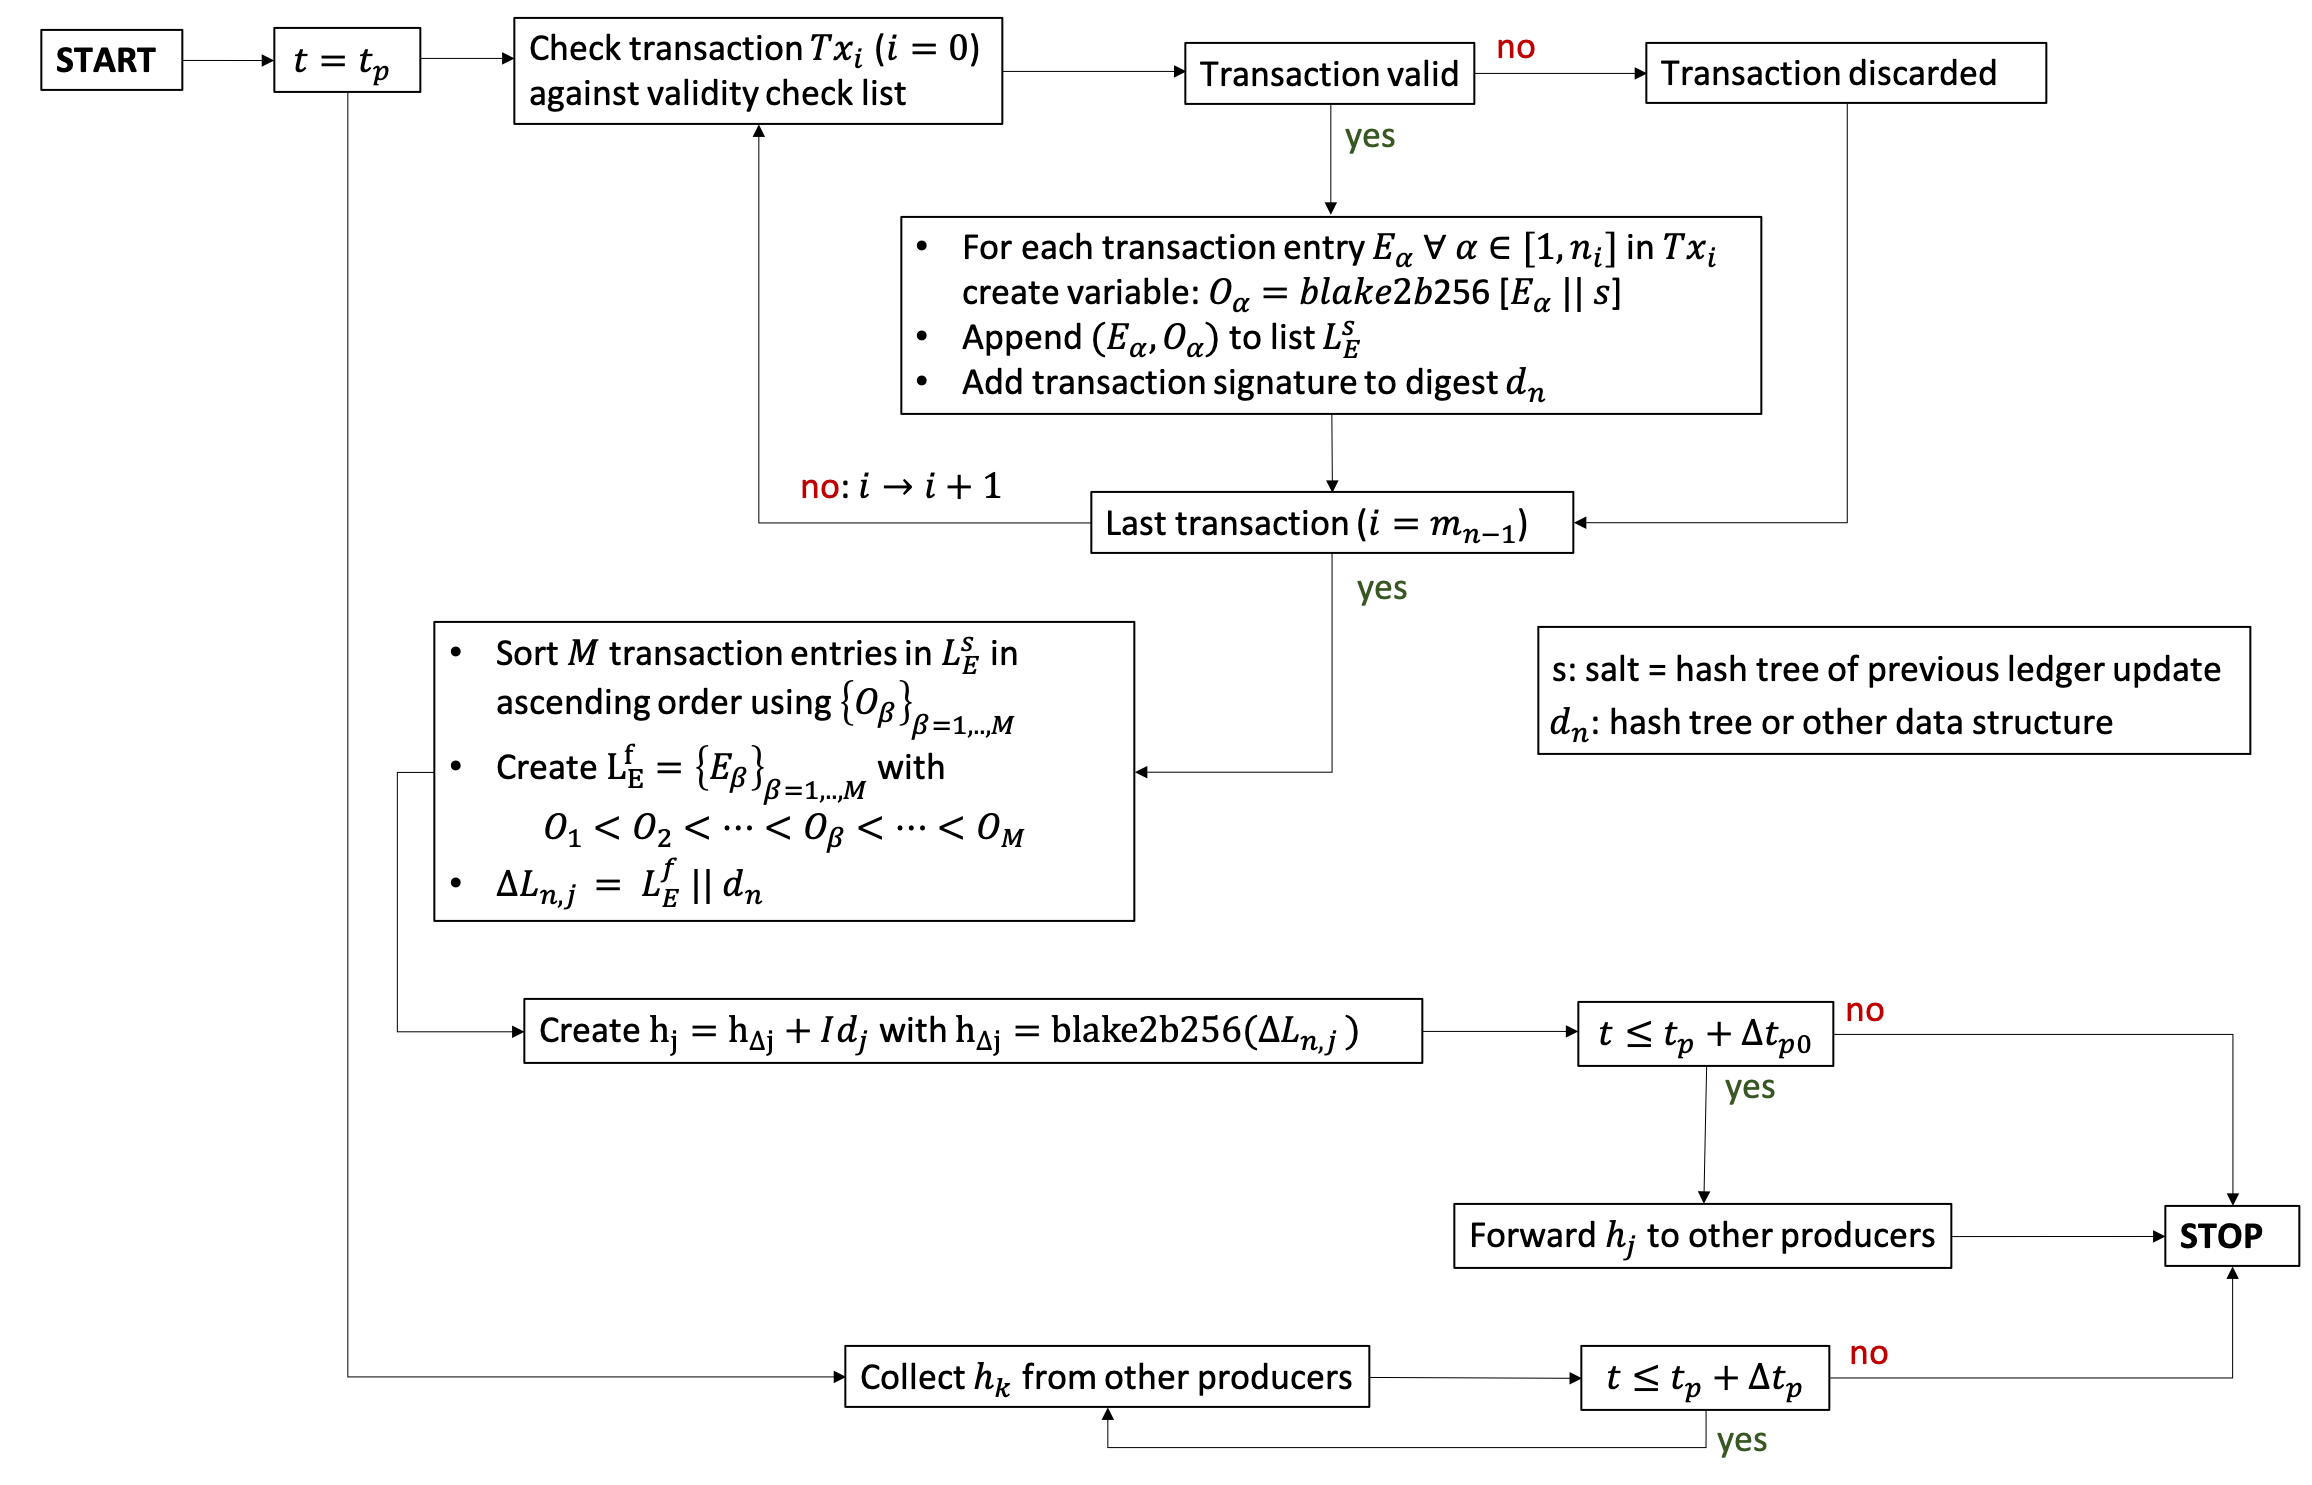
\includegraphics[width=12cm]{Figures/Local_Ledger_Computation}}
\caption{\label{fig:LLSU} Flowchart illustrated the steps followed by a producer $P_j$ node during a period of time $\Delta t_{p}$ leading to the broadcast of a local hash $h_j$.}
\end{figure}
\item At $t \leq t_p + \Delta t_{p0}$, $P_j$ broadcasts $h_j$ to the other producers in the network. Figure \ref{fig:LLSU} describes the process followed by $P_j$ to produce and broadcast $h_j$.
\end{enumerate}

\subsubsection{Local ledger state update collection}

During the first ledger cycle phase, $P_j$ collects other $\{h_k\}_{k \in P/j}$ contributions generated by its producer peers $\{P_k\}_{k \in P/j}$ in its cache. \\

At the end of the construction phase ($t = t_p + \Delta t_{p}$), $C_j$ local hashes are stored in $P_j$'s cache (including the local hash producer by $P_j$). Given the set of $P$ producers selected for the ledger cycle $\mathcal{C}_n$, the producer $P_j$ collects at most $P - 1$ contributions (\textit{e.g} $C_j = P$) with each contribution made of a local hash and a unique identifier. In an ideal world, two producers $P_j$ and $P_k$ would use the same set of transactions and as a result compute the same quantity ledger state update, leading to $\Delta L_{n,j} = \Delta L_{n,k}$. In practice, a producer may not collect exactly $P$ local hashes during $\Delta t_{p}$(\textit{e.g} $C_j \leq P$) and may not process the exact same set of transactions as its peers. The following steps describe how each producer can verify that a ledger state update has been generated by a majority of producers and generate the reward allocated to the producers. 

%%%%%%%%%%%%%%%%%%%%%%%%%%%%%%%%%%%%%

\subsection{Campaigning Phase}
\label{subsec:camp}

During the second phase (\textit{a.k.a} campaigning phase) of a ledger cycle, a producer $P_j$ designates a candidate for the correct ledger state update. At the end of the process, producers forward their proposed candidate to their peers. \\

The second phase starts at $t = t_c$ where $t_c = t_p + \Delta t_{p}$ and lasts for a period of time $\Delta t_{c}$, therefore ending at $t_c+\Delta t_{c}$.

\subsubsection{Local candidate generation and broadcast}
\label{subs:lv}
Using the $C_j$ contributions stored in its cache, $P_j$ follows a series of steps during a period of time $\Delta t_{c0}$ ($\Delta t_{c0} < \Delta t_{c}$):
\begin{enumerate}
\item $P_j$ verifies that the same local hash $h^{maj}_{\Delta j}$ is embedded in a majority $C^{maj}$ of contributions, where $h^{maj}_{\Delta j}= max[unique(h_{\Delta k})~\forall~k\in\{C_j\}]$ and $C^{maj} = count[(h_{\Delta k} = h^{maj}_{\Delta j})~\forall~k\in\{C_j\}]$. The threshold, $C_{threshold}$, to decide if a majority of producers agrees on the same ledger state update, should be strictly greater than 50\%, due to statistical consideration. The relevant variables for a producer to decide if the same ledger state update is found by a majority of producers are $C_{min}$ and $C^{maj}$. Threshold considerations are discussed in detail in section~\ref{Sec:SecLsu}. 

If $C_j > C_{min}$ and $C^{maj} > C_{threshold}$ :

\begin{itemize}
\item $P_j$ creates a list $\mathcal{L}_j(prod)$ and appends to said list the identifiers of any producer $P_k$ who forwarded a contribution $h_k$ satisfying $h_{\Delta k} = h^{maj}_{\Delta j}$.\\
If $h_{\Delta j}= h^{maj}_{\Delta j}$, $P_j$ also appends its identifier to the list $\mathcal{L}_j(prod)$.
\item The producer $P_j$ then computes the following quantity: 

\begin{equation}
\label{eq:cj}
\fbox{$c_j = h^{maj}_{\Delta j}~||~\#(L_j(prod))~||~Id_j$}
\end{equation}

Where \# represents a hash tree or some other compressed data structure of the list $L_j(prod)$. $c_j$ corresponds to $P_j$'s candidate for the most popular ledger state update. A hash tree of a list is useful to quickly verify that an object (an identifier) is included in the list. $\#(\mathcal{L}_j(prod))$ is a witness of the list of producers who correctly generated the most popular ledger state update according to $P_j$. 
\item At $t \leq t_c+\Delta t_{c0}$, $P_j$ broadcasts its candidate $c_j$ to the other producers in the network. Figure \ref{fig:computation} displays a flowchart describing the steps followed by $P_j$ to create and broadcast $c_j$.
\end{itemize}

\begin{figure}[H]
\label{fig:computation}
\center{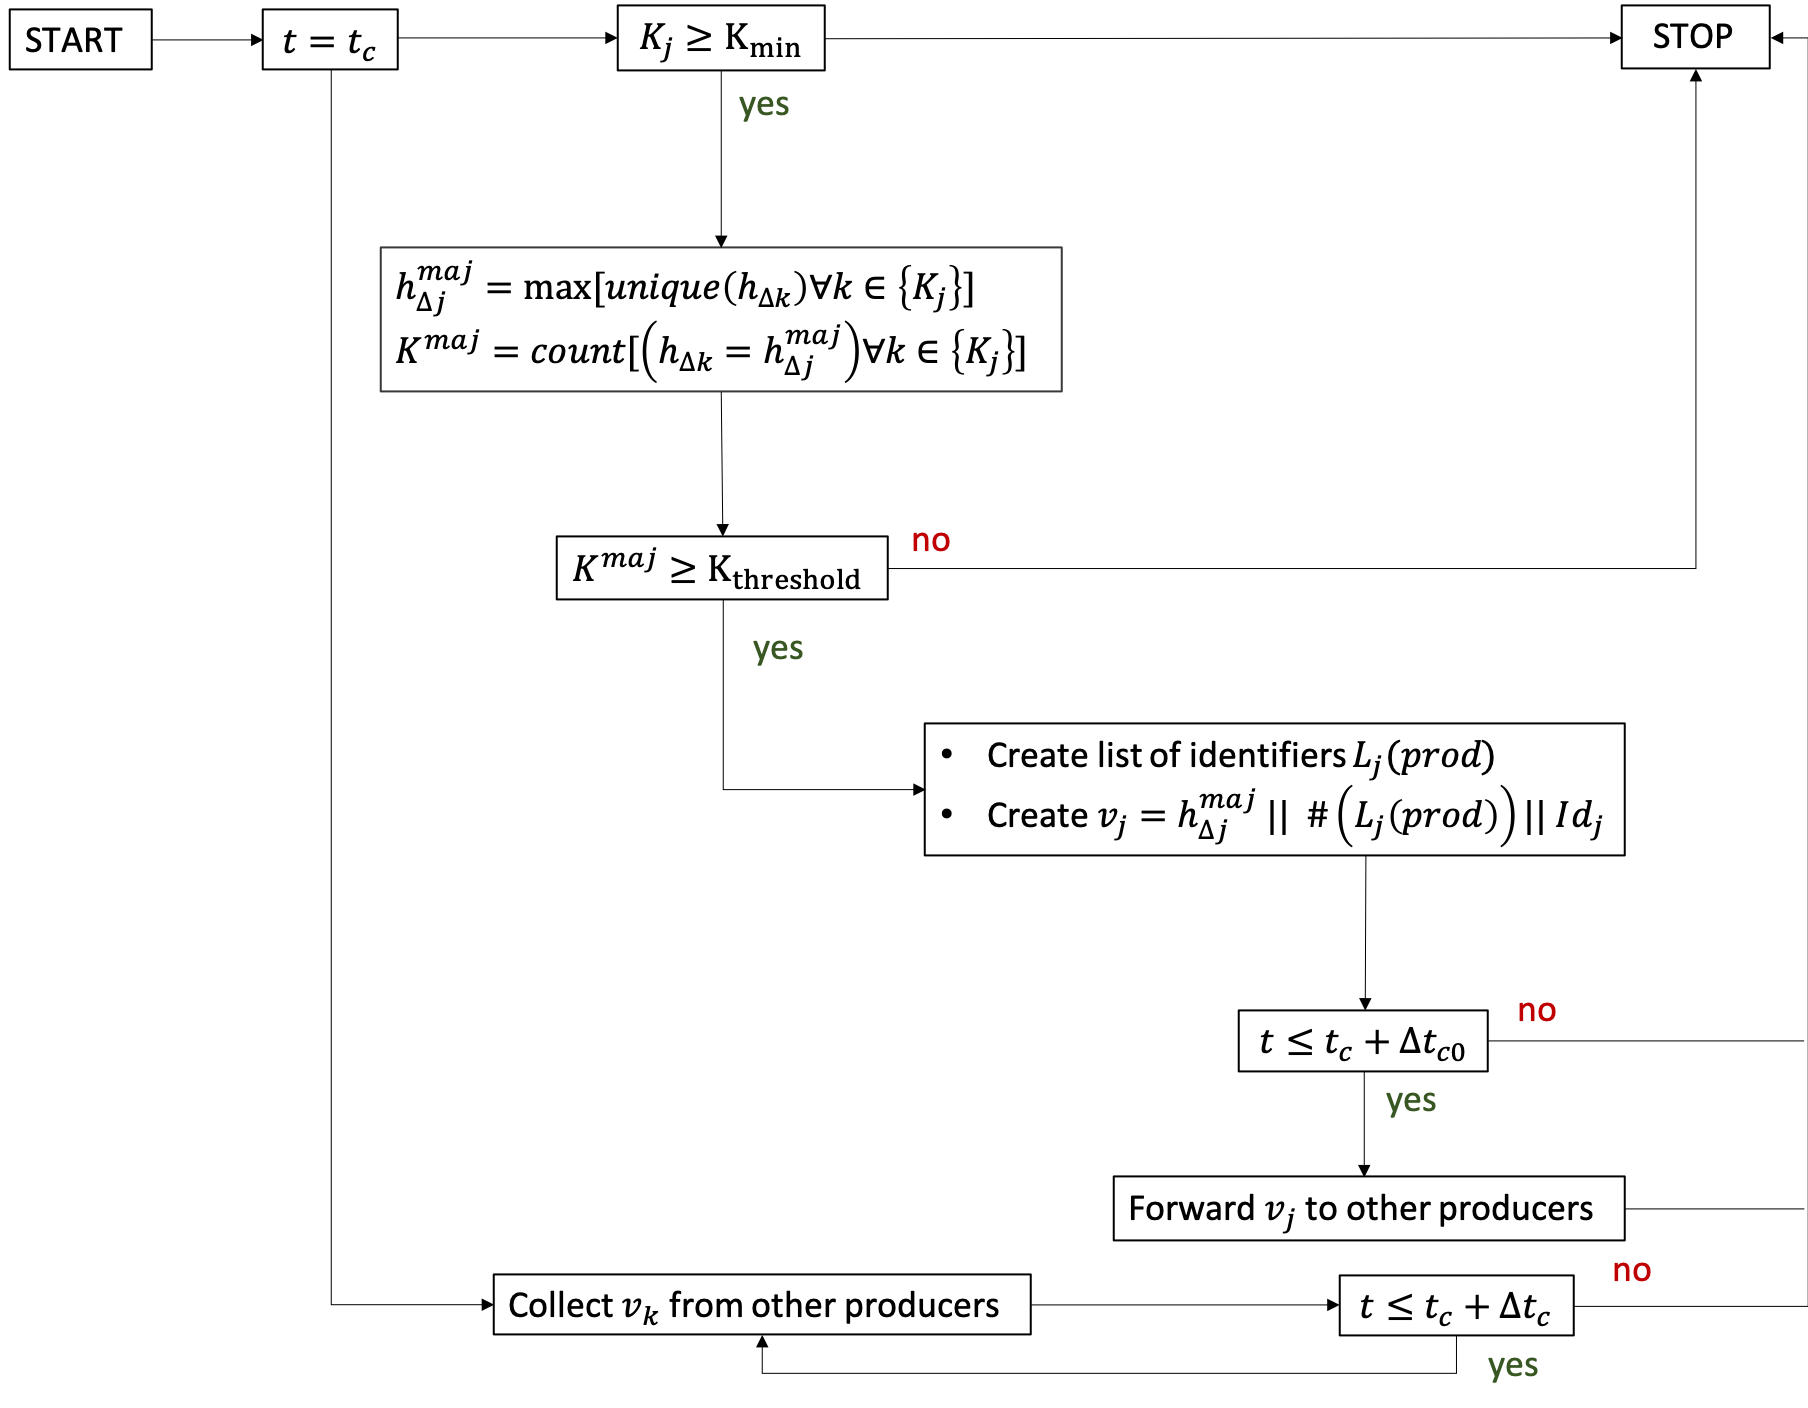
\includegraphics[width=12cm]{Figures/Local_Vote_Broadcast}}
\caption{\label{fig:computation} Flowchart illustrating the series of steps followed by a producer $P_j$ to issue a candidate $c_j$.}
\end{figure}
\end{enumerate}

\subsubsection{Local candidate collection}
Shortly after the second phase starts (at $t \approx t_c$), $P_j$ starts collecting other candidates $c_{k}$ generated by other producers $\{P_k\}_{k \in P/j}$ in its cache. The collection lasts for a period of time $\Delta t_{c}$ after which the producer holds $V_j$ candidates in its cache ($V_{min} \leq V_j \leq P$). 

\subsection{Voting Phase}
\label{subsec:vote}

During the third phase (\textit{a.k.a} voting phase) of a ledger cycle, a producer $P_j$ votes on the correct ledger state update. At the end of the process, producers forward their proposed ledger state update including a reward to some producers to their peers. \\

The third phase starts at $t = t_v$ where $t_v = t_p + \Delta t_{p} + \Delta t_{c}$ and lasts for a period of time $\Delta t_{v}$, therefore ending at $t_v+\Delta t_{v}$.


\subsubsection{Ballot generation and broadcast}
At $t = t_v$:
\begin{enumerate}
\item $P_j$ verifies that the same local hash $h^{maj}$ is embedded in a majority of candidates. With $h^{maj} = max[unique(h^{maj}_{\Delta k})~\forall~k\in\{V_j\}]$ and $V^{maj} = count[(h^{maj}_{\Delta k} = h^{maj})~\forall~k\in\{V_j\}]$, this condition is met if $V^{maj} > V_{threshold}$ (See section~\ref{Sec:SecLsu} for more explanations). 
\item The producer $P_j$ can only participate in the following steps if the local hash computed during the computation phase, $h_{\Delta j}$, is equal to $h^{maj}$. Indeed, $P_j$ needs to have knowledge of the ledger state update of which the hash was used to vote in order to proceed. 
\end{enumerate}
 
If each producer collects the local hash generated by every producer, any two producers $P_j$ and $P_k$ would build the same list of identifiers $\mathcal{L}_j(prod) = \mathcal{L}_k(prod)$. In practice, a producer may not have collected all local hashes and as a result have an incomplete list of identifiers, yet have collected enough data to be able to issue a correct vote. We mentioned how the identifier of a producer can be appended to a local hash to verify that $P_j$ is a producer node selected for the ledger cycle and evaluate the quality of work performed by $P_j$. Indeed, $Id_j$ can be used to create and add a compensation entry to the ledger state update, that rewards the producer for its work performed during the ledger cycle. The correct (complete) list of producers who successfully built the correct (dominant) ledger state update for that cycle, $\mathcal{L}_n(prod)$, is used to create these new transaction entries and append them to the final ledger state update generated for that cycle. It is therefore crucial that a majority of producers succeed in generating that list in order to generate the same final ledger state update. \\ 


The voting process thus consists in creating the final list of identifiers involved in the production of the ledger state update. As explained below the final list $\mathcal{L}_n(prod)$ is obtained by merging the partial lists included in the producers' vote. A producer $P_j$ could have produced a different hash $h_{\Delta j}$ to $h^{maj}_{\Delta j}$ yet added his identifier to $\mathcal{L}_j(prod)$ in the attempt to get some token reward allocated to producers who correctly produced the next ledger state update. In such scenario $Id_j$ would be an element of the list included in $c_j$ (or any other producer node controlled by $P_j$), but it wouldn't be included in any other list $\{\mathcal{L}_k(prod)\} \forall~k \in P/j\}$. To prevent such malicious behaviour, a rule imposes that $P_j$ only append to the final list $\mathcal{L}_n(prod)$ the identifier of a producer included in the list $\mathcal{L}_k(prod)$ of a candidate $c_k$ satisfying $h^{maj}_{\Delta k} = h^{maj}$ if and only if that identifier is included in at least $P/2$ lists $\{\mathcal{L}_{k}(prod)\}_{k=1,..,V_j}$ associated to a candidate $c_{k}$ satisfying $h^{maj}_{\Delta k} = h^{maj}$. Although this eliminates the risk of unethical behaviour from the producer, this also means that there would be little incentive for a producer to broadcast its vote if its identifier was not included in $\mathcal{L}_n(prod)$. However, the probability that a producer compiles the correct final list $\mathcal{L}_n(prod)$ strongly depends on the number of votes collected. The more votes collected by a producer, the greater the probability that said producer will compile the complete final list. Although a producer may not have produced the correct local ledger state update, participating in the voting process is, therefore, an important contribution to the overall consensus protocol and should entitle the producer to some reward. To that end a producer $P_j$ can use the identifier of other producers included in their vote and create a second list $\mathcal{L}_j(vote)$ to account for their participation in the voting process. \\
 
$P_j$ follows a series of step for a period of time $\Delta t_{v0}$ ($\Delta t_{v0} < \Delta t_{v}$):

\begin{enumerate}
\item $P_j$ creates a new list $\mathcal{L}_j(vote)$ and appends to said list the identifier of any producer $P_k$ who forwarded a candidate $c_k$ satisfying $h^{maj}_{\Delta k} = h^{maj}$.
\item $P_j$ creates the final list $\mathcal{L}_n(prod)$ and appends to said list the identifier of a producer included in the list $\mathcal{L}_k(prod)$ of a candidate $c_k$ satisfying $h^{maj}_{\Delta k} = h^{maj}$ if and only if that identifier is included in at least $P/2$ lists $\{\mathcal{L}_{k}(prod)\}_{k=1,..,V_j}$ associated to a candidate $c_{k}$ satisfying $h^{maj}_{\Delta k} = h^{maj}$. 
\item $P_j$ then creates a list $L_{CE}$ of compensation entries for each producer whose identifier is included in $\mathcal{L}_n(prod)$. Each producer receives $x_h$ tokens. Assume that $Y_h \leq P$ identifiers are included in $\mathcal{L}_n(prod)$ and $X$ is the total number of tokens injected per cycle for the pool of $P$ producers. The quantity $x_h$ is defined such that $Y_hx_h = f_{prod}X + x_f$ where $x_f$ represents the total number of fees collected from the $m_{n-1}$ transactions and $f_{prod}$ represents the fraction of new tokens injected per cycle and distributed to the producers who built the correct ledger state update. The remaining $(1-f_{prod})X$ tokens are distributed to other contributing nodes in the network. A part of this remainder goes to the producers who voted correctly on the previous ledger cycle update. Let $\mathcal{L}_{n-1}(vote)$ be the list of the identifiers of producers who voted correctly on the previous ledger cycle update $\mathcal{C}_{n-1}$. We later demonstrate how such a list is derived during a ledger cycle. For now, let's assume that $L_{CE}$ includes compensation entries for producers involved the production of the ledger state update for this ledger cycle $\mathcal{C}_n$ and the producers involved in the voting process of the precedent cycle $\mathcal{C}_{n-1}$. 
\item $P_j$ then creates the final ledger state update for $\mathcal{C}_n$ including the reward allocated to the producers for their contribution:
\begin{center}
$\mathbf{LSU_j = L^f_E~||~d_n~||~L_{CE}}$
\end{center}
$P_j$ then computes its final vote (or ballot):
\begin{equation}
\label{eq:vj}
\fbox{$v_j = \mathcal{H}(LSU_j)~||~\#(\mathcal{L}_j(vote))~||~Id_j$}
\end{equation}

which includes a partial list of identifiers of producers who designated the correct candidate for the ledger state update $h^{maj}$. 

\item $P_j$ then forwards $v_j$ to the other producers and collect the votes issued by its peers. Figure \ref{fig:Vot} illustrates the different steps followed by $P_j$ during the voting phase.
\begin{figure}[H]
\label{fig:Vot}
\center{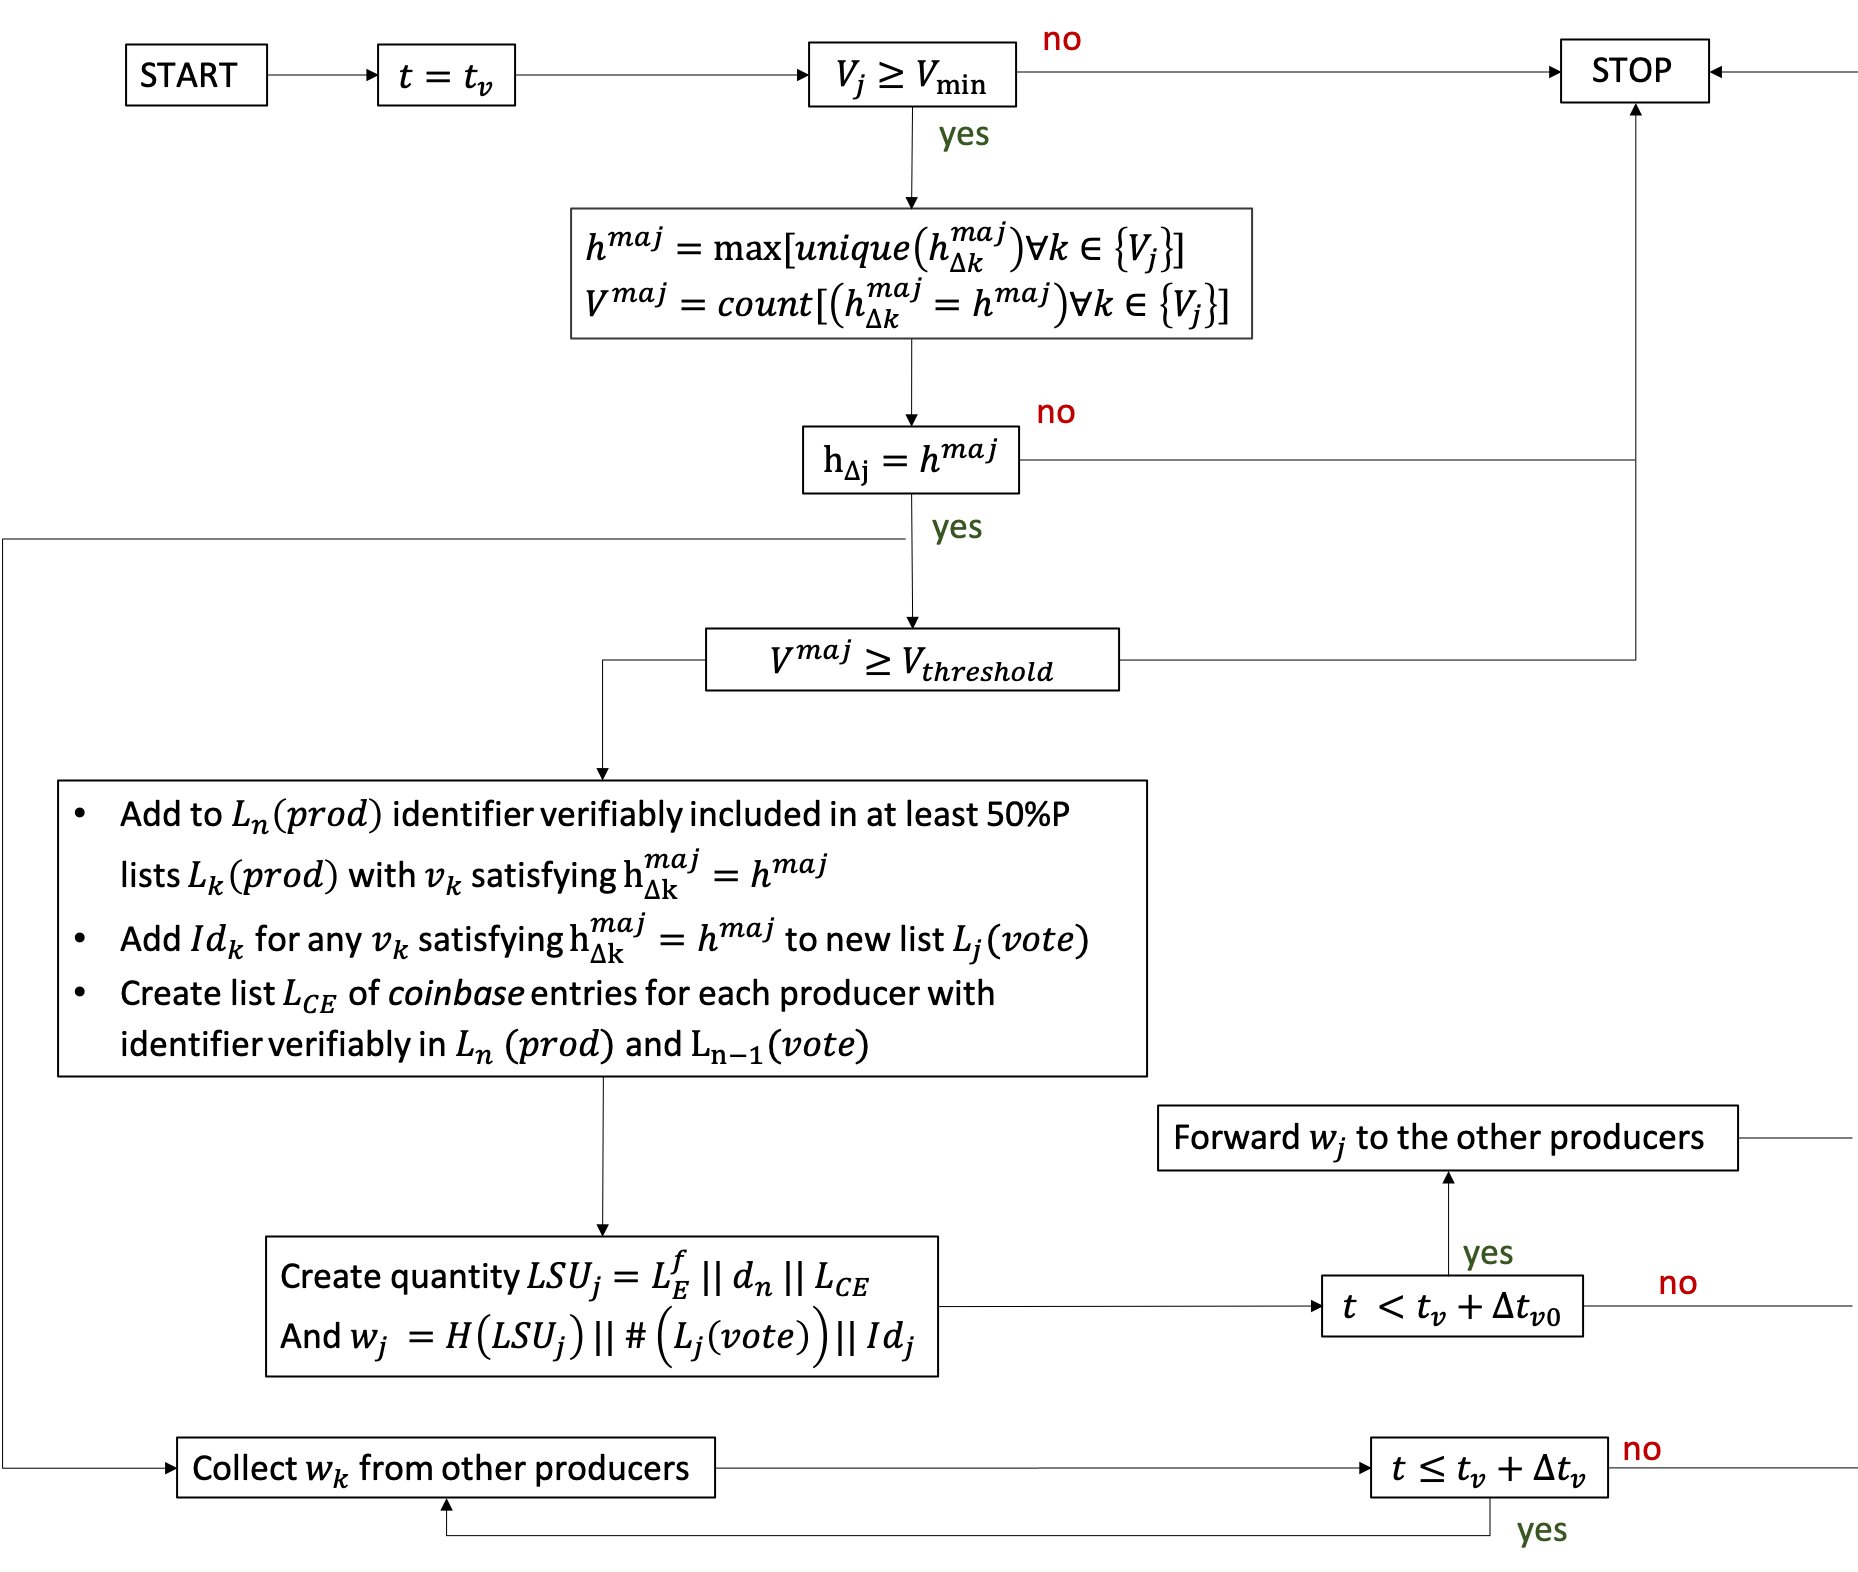
\includegraphics[width=11cm]{Figures/Global_Vote_Broadcast}}
\caption{\label{fig:Vot}Flowchart illustrating the series of steps followed by a producer $P_j$ during the voting phase of the ledger cycle.}
\end{figure}
\end{enumerate}


\subsubsection{Ballot collection}
During the voting phase, the producer $P_j$ collects the votes broadcast by its peers. At the end of the voting phase ($t = t_v+\Delta t_{v}$), the producer $P_j$ holds $U_j$ final votes in its cache with $U_j \leq C_n$ where $C_n \leq P$ is the actual total number of producers who correctly computed $h^{maj}$.

%%%%%%%%%%%%%%%%%%%%%%%%%%%%%%%%%%%%%

\subsection{Synchronisation Phase}
\label{subsec:sync}
\subsubsection{Final ledger state update generation and broadcast}

The last phase (\textit{a.k.a} synchronisation phase) of a ledger cycle starts at $t = t_s$, with $t_s = t_{n,0} + \Delta t_{p} + \Delta t_{c}+ \Delta t_{v}$, and lasts for a period of time $\Delta t_{s}$, therefore ending at $t_s+\Delta t_s = t_{n,0} + \Delta t_{cycle}$.

During a period of time $\Delta t_{s0} < \Delta t_{s}$, $P_j$ executes the following steps:

\begin{enumerate}
\item $P_j$ defines the ledger state update $\Delta L_n$ for the cycle $\mathcal{C}_n$ as:\\
 $\mathcal{H}(\Delta L_n) = max[unique(\mathcal{H}(LSU_k))~\forall~k\in\{U_j\}]$ and the associated number of votes collected: $U^{maj} = count[(\mathcal{H}(LSU_k) = \mathcal{H}(\Delta L_n))~\forall~k\in\{U_j\}]$ and verifies that $U^{maj}> U_{threshold}$.
\item $P_j$ creates a new list $\mathcal{L}_{n}(vote)$ and appends to $\mathcal{L}_{n}(vote)$ the identifier of a producer included in the list $\mathcal{L}_{k}(vote)$ of a vote $v_k$ satisfying $\mathcal{H}(LSU_k) = \mathcal{H}(\Delta L_n)$ if and only if the identifier is included in at least $C_n/2$ lists $\{\mathcal{L}_{k}(vote)\}$ associated to a vote $v_{k}$ satisfying $\mathcal{H}(LSU_k) = \mathcal{H}(\Delta L_n)$. Note that $C_n$ can be easily computed as it corresponds to the number of producer identifiers who correctly computed the ledger state update and are therefore included in $\mathcal{L}_{n}(prod)$.
\begin{comment}
\item $P_j$ then creates the following quantities:
\begin{equation} 
\fbox{$\mathbf{H_{j} = \mathcal{H}(\Delta L_n)~||~\#(\mathcal{L}_{n}(vote))~||~Id_j}$}
\label{eq:Hj}
\end{equation}
\end{comment}
\item If $P_j$ generated the correct ledger state update $\Delta L_n$, it can write it to DFS which will return it with a content based address $\mathcal{A}_n$. 
\item A Producer $P_j$ then creates the following quantity:
\begin{equation} 
\fbox{$\mathbf{H_{j} = \mathcal{A}_n~||~\#(\mathcal{L}_{n}(vote))~||~Id_j}$}
\label{eq:Hj}
\end{equation}
%The producer then broadcasts $H_j$ to the network.% Worker nodes, as well as DFS nodes collect the quantities $\{H_k\}_{\forall~k\in\{P\}}$. %Upon receiving individuals quantities, workers store $\#(\mathcal{L}_{n}(vote))$ in their mempool. 
\end{enumerate}


\subsubsection{Ledger state synchronisation across the network}

During the time period [$t_{s}, t_s + \Delta t_{cycle}$], user nodes collect $\{H_k\}_{\forall k \in P}$ quantities broadcast by the producers. 
By extracting the identifier $Id_k$ embedded in any collected quantity $H_k$, a user node can easily compile a list of producer identifiers having broadcast the same quantity $\mathcal{H}(\Delta L_n)$ (concatenated with the same list $\mathcal{L}_{n}(vote)$). Upon receiving $x > P/2$ identical addresses $\{\mathcal{A}_k = \mathcal{A}_n\}_{k \in x}$, the user nodes can read the common address content ($\Delta L_n$) from DFS. Using $\Delta L_n$ a user node can safely synchronise their local copy of the ledger and write it to their DFS if not already done. The balance of accounts stored on the ledger are updated and the producers effectively collect their rewards.\\


Worker nodes also store the list $\mathcal{L}_{n}(vote)$ embedded in each $H_k$ quantity. If selected to be a producer for the next cycle $\mathcal{C}_{n+1}$, a worker can use it to generate the reward allocated to the producers who correctly voted for the accurate ledger state update during the ledger cycle $\mathcal{C}_{n}$.\\


\begin{comment}
Producers having generated the correct ledger state update $\Delta L_n$ can write it to DFS. 


During the time period [$t_{s}, t_s + \Delta t_{cycle}$], worker nodes, as well as DFS nodes collect $\{H_k\}_{\forall k \in P}$ quantities broadcast by the producers. 
By extracting the identifier $Id_k$ embedded in any collected quantity $H_k$, a DFS node can easily compile a list of producer identifiers having broadcast the same quantity $\mathcal{H}(\Delta L_n)$ (concatenated with the same list $\mathcal{L}_{n}(vote)$). Producers having generated the correct ledger state update $\Delta L_n$ can forward it to DFS nodes.
User nodes can collect the  content based address from producer nodes. 

The nodes which have the correct delta can all write it to the DFS. It will return them with a content based address, which is a sort of hash. Then if you dont have the hash (because you didn't have the content) you can collect it from a majority x > P/2 and read its content from the DFS. That is my understading.
Once a DFS node has collected $x \geq P/2$ identical hash values, they can accept any $\Delta L_n$ value matching $\mathcal{H}(\Delta L_n)$. User nodes can then request the ledger state update $\Delta L_n$ from DFS nodes and safely synchronise their local copy to the ledger. The balance of accounts stored on the ledger are updated and the producers effectively collect their rewards. \\

\end{comment}

Figure~\ref{fig:cycle} summarises the different phases of the ledger cycle.\\

The various parameters and thresholds mentioned in this chapter and their impact on the levels of security and confidence in the successful production of a ledger state update are discussed in section~\ref{Sec:SecLsu}.
\newpage
\begin{landscape}
\begin{figure}
\center
    \includegraphics[width=22cm,height=42cm,keepaspectratio]{Figures/Catalyst_cycle}
    \caption{\label{fig:cycle}Illustration of the different phases followed by a producer during a ledger cycle.}
\end{figure}
\end{landscape}



%%%%%%%%%%%%%%%%%%%%%%%%%%%%%%%

\chapter{Catalyst at Large Scale} \label{Cha:Sha}

\textbf{section in progress}\\



%%%%%%%%%%%%%%%%%%%%%%%%%%%%%%%

\chapter{Benchmarking} \label{Cha:Ben}

Work in progress

%%%%%%%%%%%%%%%%%%%%%%%%%%%%%%%

\chapter{Security} \label{Cha:Sec}

Whenever financial value is stored on a distributed system, there will be greater incentive to attack the system in the attempt to take control of financial assets or simply disrupt the system to create or destroy existing assets. %This is why security against attack on DLT must be of the most grave importance. 
With no centralised entity to control access and check validity it is up to the peers on the network to ensure its security. Through consensus and the underlying protocols of the network a secure environment must be created to allow transactions to take place in a trust-less environment. 


\section{Security of the Consensus Mechanism I }\label{Sec:ConSec}

The primary attack of concern for all blockchain and DLT platforms is the subversion of their consensus protocol and is generally referred as a 51\% attack. Such attack is made possible when an entity or group of entities collude to have enough influence on the network to produce a block or ledger state update with invalid transactions, in the attempt to alter the ledger integrity. Depending on the protocol, the influence can be in computing power or number of nodes and exceeds 50\% of the relevant resource.  \\

An attack could be performed for many reasons aside attempting to steal money from a network, including to discredit or shake trust in a network. A consequence of a successful attack would likely be to reduce token prices. Although there is no tangible proof of this, it could explain why 51\% attacks are not too common. Nevertheless, it remains important to prevent and mitigate the risk of an attack as much as possible.\\

The probability of a 51\% attack ($P_{51}$) typically depends on the algorithm used to produce a valid block or ledger update.When considering PoW-based algorithms, $P_{51}$ can be expressed as a function of the hash rate of network nodes.  Since the consensus-based protocol on the Catalyst network as laid out in section \ref{Cha:CM} does not rely on solving a cryptographic puzzle, the concept of hash rate of nodes involved in the ledger state update is not relevant to quantify the probability or the cost of an attack on Catalyst network. The number of nodes involved in the production of a ledger state update is however relevant, as explained in this section. \\ 

The probability of a successful 51\% attack on Catalyst network implies that a malicious entity (or group of entities) succeeds in controlling more than half the producer nodes selected to produce the ledger state update during a ledger cycle, giving that entity the power to tamper with the ledger state. The probability $P_{51}$ depends on the following parameters:
\begin{itemize}
\item $N$ : the total number of nodes in the worker pool. 
\item $P$ : the subset of worker nodes selected to perform work for one ledger cycle ($P \leq N$).
\item $O$ : the number of malicious nodes in the worker pool ($0 \leq O \leq N$). This is a total subset of malicious nodes colluding to perform an attack on the network.
\item $p$ : the number of malicious nodes in the subset $P$ of producers. ($0 \leq p \leq P$).
\end{itemize}
An attack can be considered successful for any value $p \in [p_0,P]$ where $p_0 = P/2 + 1$ which is equivalent to $p > 50\%P$. When $P \approx N$, \textit{i.e.} the number of producers selected during a ledger cycle is very close to the total number of nodes in the worker pool, the absence of a randomness element in the selection of $P$ producers  makes it easy to compute the probability of a successful attack on the network: $P_{51} \approx O/N$. A malicious entity would know exactly when an attack can successfully be performed, that is when $O > N/2$. \\

When $N \gg P$, $P_{51}$ can there be expressed by the discrete sum:
\begin{equation}
\label{eq:1}
P_{51} =  \sum_{p=p_0}^{P} P_{A}(p)
\end{equation}
where $P_{A}(p)$ represents the probability of having $p$ malicious nodes in the set $P$. When the ratio between the total number of nodes $N$ and the number of nodes $P$ is large ($N > 20\times P$) it can be expressed as follows: 
\begin{equation}
\label{eq:2}
P_{A}(p) = \frac{\overbrace{\left( \begin{array}{c} O \\
p \end{array} \right)}^\text{A} 
\overbrace{\left( \begin{array}{c} N - O \\ P - p \end{array} \right)}^\text{B}}{\underbrace{\left( \begin{array}{c} N \\
P \end{array} \right)}_\text{C}}
\end{equation}
$A$ represents the number of possible combinations for choosing $p$ nodes from $O$ malicious nodes. $B$ represents the number of possible combinations for choosing good (non-malicious) nodes for the remaining $N-0$ nodes in the worker pool. Finally, $C$ corresponds to the number of available combinations for choosing $P$ nodes from the pool of $N$ nodes.\\
\\
In equation \ref{eq:2}, $P_A(p)$ is the probability mass function of a hypergeometric distribution over the set of parameters $\{N,O,P\}$. Note that such expression is valid for $max(0,O+P-N) \leq p \leq min(O,P)$. \\

There are two main arguments behind having a large number of $N$ nodes:

\begin{itemize}
 \item To account for the fact that most nodes with sufficient resources may want to join the worker pool and receive tokens as reward for their contribution to the ledger state management
\item To make it increasingly costly for any malicious entity to control more than half the nodes.
\end{itemize}

\begin{comment}
As explained in section~\ref{Sec:Reg}, prior to joining the worker pool, nodes are part of a work queue. Nodes in the worker pool are granted a work pass valid for finite period time. When a node $W_j$ joins the worker pool, it is granted a work pass defined by a decay rate $\lambda_j$. Similarly to unstable nuclear elements the work pass has a 50\% chance to remain valid after $W_j$ sits in the worker pool for a period of time $ln(2)/\lambda_j$. The decay rate is not fixed over time but instead can very depending on the quality of work produced by $W_j$ when selected to be a producer. The quality of work performed by a producer during a ledger cycle $\mathcal{C}_n$ can be estimated by verifying if the producer identifier is found in the lists $\mathcal{L}_n(prod)$ and $\mathcal{L}_n(vote)$. If the identifier is found in one of the two lists or none, the decay rate increases. $\lambda_j$ can also vary to account for the demand of work, \textit{i.e.} the length of the work queue, although a threshold is considered to mitigate the risk of a malicious entity (or group of entities) trying to simulate a highest demand for work than reality.
\end{comment}
As explained in section~\ref{Sec:Reg}, prior to joining the worker pool, nodes are part of a work queue. Nodes in the worker pool are granted a work pass valid for finite period time. As a result, a varying number of nodes leaves the worker pool at each ledger cycle. Although the size of the worker pool might be constant ($N$ nodes), the selection of nodes actually forming the worker pool changes over time. The mechanism to define a score for nodes in the work queue is designed to prevent malicious nodes from gaining control of a large fraction of worker nodes. Nevertheless, as we derive the probability $P_{51}$ in this section, we must stress that the fraction $O/N$ may change (increase or decrease) over time and should be taken into account if computing the probability over a series of ledger cycles.\\

When $N \gg P$ the probability of a successful attack can therefore be estimated using the cumulative hypergeometric distribution function (CDF) for $p \in [p_0,P]$. In this paper, we provide probability estimate obtained using $scipy.stats$ Python library. The graphs presented are obtained using $matplotlib.pyplot$ library. Rather than computing the CDF, the probability measurements are obtained using the survival probability (SDF), which is the inverse of CDF but is known to provide more accurate results\footnote{See https://docs.scipy.org/doc/scipy-0.14.0/reference/generated/scipy.stats.hypergeom.html for more details.}. \\

As an example, assume a rather large number of nodes in the worker pool, $N = 20,000$, out of which $5\%$ are selected as producers for a given cycle ($P = 1,000$). 
Further assume a ratio $O/N=20\%$, \textit{e.g.} $1$ every $5$ nodes in the worker pool is controlled by a malicious entity ($O=4000$). The probability of a successful attack is calculated using the SDF of an hypergeometric distribution using these set of parameters and amounts to: $P_51 = 1-SDF(20000,4000,1000) \approx 10^{-9}\%$. For the same set $(N,P)$, the probability of a successful attack reaches $0.04\%$ for $S=45\%$ of malicious nodes in the worker pool. 

Figure \ref{fig:P} shows the probability of a successful control of more than 50\% of the producers as a function of the number of producers for four different worker pool sizes and two attack scenarios: when a malicious entity controls $O/N = 45\%$ of the worker nodes in blue, and in orange when a malicious controls $O/N = 35\%$ of the worker nodes in blue. For $N=20000$, the probability remains below $10^{-9}$ if $P < \approx 4000$ while for a smaller worker pool size ($N=5000$), the ratio $P/N$ must be at close to 50\% to prevent a successful control of more than 50\% of the producers. 

\begin{figure}[H]
\centering
 \begin{subfigure}[b]{0.45\textwidth}
        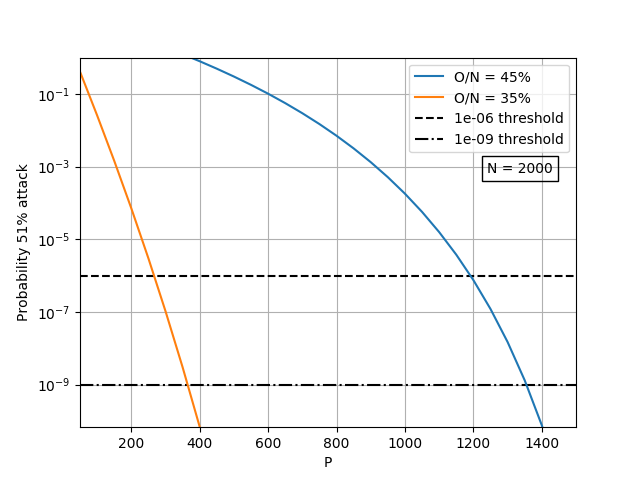
\includegraphics[width=\textwidth]{Figures/Prob51_vs_P_N2000_O35_to_45}

        \renewcommand{\thesubfigure}{a}
     \caption{$N = 2000$}
        \label{fig:N2000}
    \end{subfigure}
    \begin{subfigure}[b]{0.45\textwidth}
        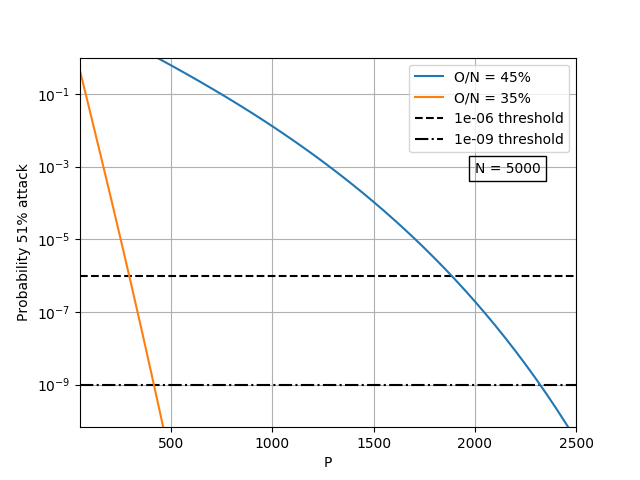
\includegraphics[width=\textwidth]{Figures/Prob51_vs_P_N5000_O35_to_45}
   
        \renewcommand{\thesubfigure}{b}
        \caption{$N = 5000$}
        \label{fig:N5000}
    \end{subfigure}
        \begin{subfigure}[b]{0.45\textwidth}
        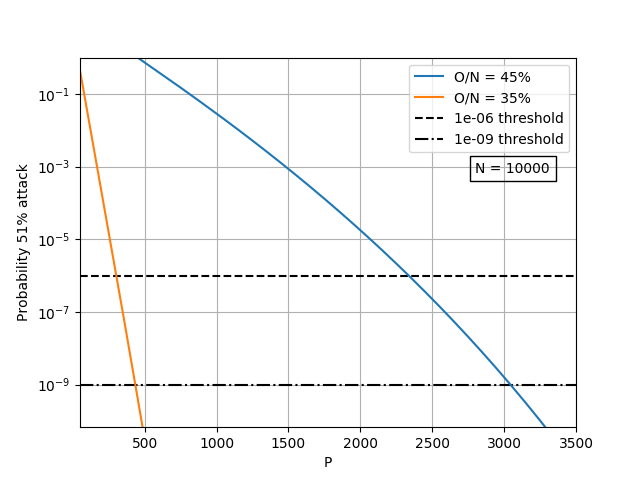
\includegraphics[width=\textwidth]{Figures/Prob51_vs_P_N10000_O35_to_45}
   
        \renewcommand{\thesubfigure}{c}
        \caption{$N = 10000$}
        \label{fig:N10000}
    \end{subfigure}
        \begin{subfigure}[b]{0.45\textwidth}
        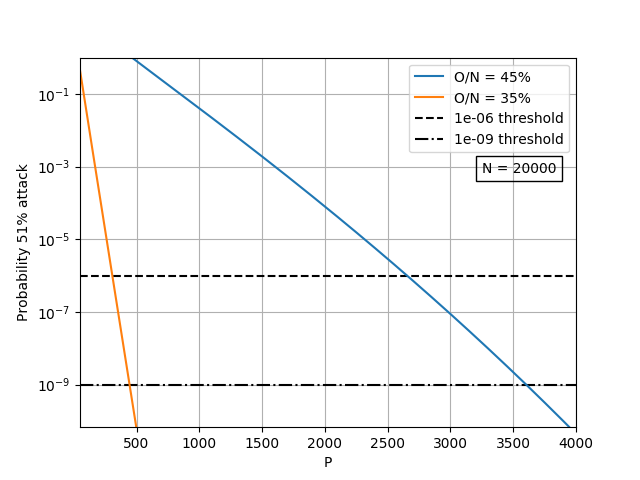
\includegraphics[width=\textwidth]{Figures/Prob51_vs_P_N20000_O35_to_45}
   
        \renewcommand{\thesubfigure}{d}
        \caption{$N = 20000$}
        \label{fig:N=20000}
    \end{subfigure}
\caption{Probability of 51\% attack as a function of P for various worker pool size ($N=\{2000, 5000, 10000, 20000\}$) when a malicious entity controls $O/N = 45\%$ of the worker nodes in blue, and in orange when a malicious controls $O/N = 35\%$}\label{fig:P}
\end{figure}    

Figure \ref{fig:threshV} displays the minimum ratio $P/N$ required to maintain a probability below $10^{-6}$ and $10^{-9}$ for various malicious scenario ($O/N$ ratio between 30\% and 45\%) . This shows that as $N$ increases the required $P/N$ ratio required for the same security level decreases. 

\begin{figure}[H]
	\centering
	\begin{subfigure}[b]{0.45\textwidth}
		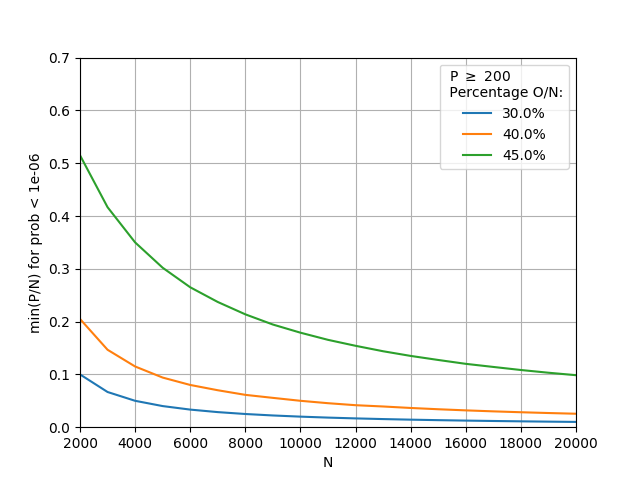
\includegraphics[width=\textwidth]{Figures/PoN_vs_N_Thre_Prob51_10em6_O30_to_45}
		
		\renewcommand{\thesubfigure}{a}
		\caption{Prob. Attack = $10^{-6}$}
		\label{fig:N20-50}
	\end{subfigure}
	\begin{subfigure}[b]{0.45\textwidth}
		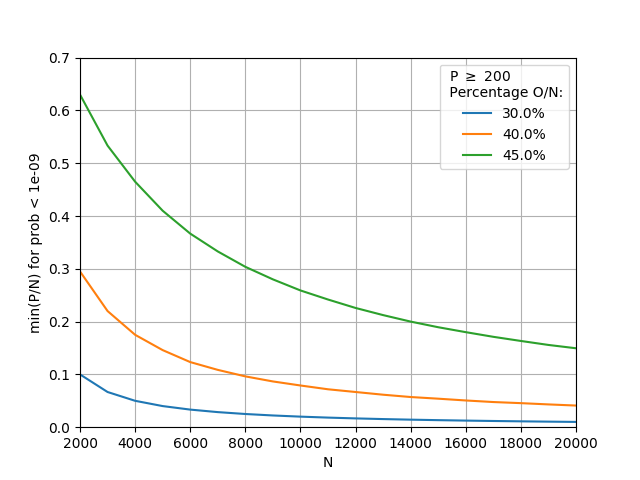
\includegraphics[width=\textwidth]{Figures/PoN_vs_N_Thre_Prob51_10em9_O30_to_45}
		
		\renewcommand{\thesubfigure}{b}
		\caption{Prob. Attack = $10^{-9}$}
		\label{fig:N50-100}
	\end{subfigure}
\caption{\label{fig:threshV} This graph shows the $P/N$ ratio required for a probability of a 51\% attack of less than $10^{-6}$ on a validation cycle versus $N$. This is shown against various $O/N$ ratio. }
\end{figure}

This series of graphs gives a good indication on what pair of parameters ($N,P$) to consider for a high resilience to 51\% attack. Given a number of nodes in the worker pool, we can deduce the number of producer nodes to select during one ledger cycle. Inversely, given a selected number of producers for a ledger cycle, we can define a minimum size for the worker pool. As detailed in the next section, the number of producers selected for a ledger cycle is important to ensure that a consensus can be reached on the correct ledger state update to distribute to the rest of the network.

%In section~\ref{subsec:comp}, we consider the fact that a producer may not collect exactly $P$ local hashes during the first ledger cycle phase. We argue that a threshold $P_{min}$ should apply to decide whether a majority of producers build the same local hash. 


\section{Security of the Consensus Mechanism II }\label{Sec:SecLsu}

The previous section discusses the level of security against 51\% attack when a malicious entity controlling more than half the producer nodes can attempt to tamper with the ledger update. Specifically, the security of the consensus mechanism is considered as a function choice of parameters ($P,N$). As $N$ becomes large and the ratio $P/N$ is low, it becomes very unlikely for a malicious entity to gain control of the worker pool, notwithstanding an increasingly expensive cost of attack. \\

In this section, we explore the confidence level associated with the production of a ledger state update. During the last phase of the consensus mechanism, each node on the network updates their local copy of the ledger with what they perceive as being the correct ledger state update generated by the producers. Each user node must collect $x > P/2$ identical hashes from the producers to safely conclude that a consensus was reached amongst the producers. Recall that a producer $P_j$ broadcasts $\mathcal{H}_{j} = A_n~||~\#(\mathcal{L}_{n}(vote))~||~Id_j$ to the network. The producer identifier $Id_j$ is used by a user node to distinguish between the DFS content-based address generated by two producers. The correct address $\mathcal{A}^c(\Delta L_n)$ is thus defined by $\mathcal{A}^c(\Delta L_n) = max[unique(H_k~/|~\#(\mathcal{L}_{n}(vote))~Id_k)~\forall~k\in\{P\}]$ with $/|$ denoting a removal function, and $x = count[(H_k~/|~\#(\mathcal{L}_{n}(vote))~||~ Id_k = \mathcal{A}^c(\Delta L_n))~\forall~k\in\{P\}]$. Note that if $x=P$, all producers agree on the correct ledger state update for cycle $\mathcal{C}_n$. \\

As laid out in section~\ref{Sec:Dem}, a producer executes a series of steps in each phase of the consensus mechanism in a consecutive manner. The producer can only move to a phase if a set of conditions are fulfilled in the previous phase. For a producer $P_j$, the first three phases consist of generating a quantity $\alpha_j$ that obeys certain criteria, and then broadcasting it to its producer peers while collecting the quantities $\alpha_k$ produced and broadcast by other producers $\{P_k\}_{k\in P/j}$:
\begin{enumerate}
\item \textbf{Construction phase: $\alpha_j = h_j$} \\
 $h_j$ is the hash of the ledger state update (excluding any compensation entry) generated by $P_j$, using the set of transactions stored in its mempool, concatenated with its identifier $Id_j$ (see equation~\ref{eq:hj}): $h_j = h_{\Delta j}~||~Id_j$. 
\begin{description}
\item[Participation] All producers $\{P_j\}_{\forall j \in P}$ participate in the construction phase. 
\item[Time] $h_j$ must be broadcast before $t_p + \Delta t_{p0}$. Other local hashes are collected during the time period [$t_p, t_p + \Delta t_{p}$].
\item[Quality] Each transaction included in the ledger state update must verify a list of validity checks (see section~\ref{Sec:Val}). 
\end{description}

\item \textbf{Campaigning phase}: $\alpha_j = c_j$\\
$c_j$ is the ledger state update candidate generated by $P_j$ (see equation~\ref{eq:cj}):\\
$c_j = h^{maj}_{\Delta j}~||~\#(L_j(prod))~||~Id_j$ with $h^{maj}_{\Delta j}$ the hash of the most common ledger state update found by $P_j$ given the set of local hashes collected during the construction phase. $L_j(prod)$ is the partial list of identifiers compiled by $P_j$ which includes the identifier of any producer having broadcast a local hash corresponding to the most common ledger state update.
\begin{description}
\item[Participation] All producers $\{P_j\}_{\forall j\in P}$ participate in the campaigning phase. 
\item[Time] $c_j$ must be broadcast before $t_c + \Delta t_{c0}$. Other candidates are collected during the time period [$t_c, t_c + \Delta t_{c}$].
\item[Quality] 
\begin{itemize}
\item The number $C_j$ of local hashes collected by $P_j$ must verify $C_j \geq C_{min}$.
\item The number of identical local hashes $C^{maj} = count[(h_{\Delta k} = h^{maj}_{\Delta j})~\forall~k\in\{C_j\}]$ must verify $C^{maj} \geq C_{threshold}$.
\end{itemize}
\end{description}

\item \textbf{Voting phase}: $\alpha_j = v_j$\\
$v_j$ is the vote generated by $P_j$ (see equation~\ref{eq:vj}): $v_j = \mathcal{H}(LSU_j)~||~\#(\mathcal{L}_j(vote))~||~Id_j$ with $LSU_j = L^f_E~||~d_n~||~L_{CE}$ the candidate of the ledger state update locally elected by $P_j$, which includes the compensation entries for the producers  $\{P_k\}_{\forall j\in C_n}$ who generated a local hash verifying $h_k = \mathcal{H}(L^f_E~||~d_n)$. 
$L_j(vote)$ is the partial list of identifiers compiled by $P_j$ which includes the identifier of any producer having broadcast a candidate corresponding to the most common ledger state update. $L_{CE}$ is the list of compensation entries created using the identifiers included in $L_n(prod)$, the complete and final list of $C_n$ producers having broadcast a local hash corresponding to the most common ledger state update.
\begin{description}
\item[Participation] Only producers finding a $h^{maj} = max[unique(h^{maj}_{\Delta k})~\forall~k\in\{V_j\}]$ satisfying $h^{maj} = h_j$ participate.
\item[Time] $v_j$ must be broadcast before $t_v + \Delta t_{v0}$. Other votes are collected during the time period [$t_v, t_v + \Delta t_{v}$].
\item[Quality] 
\begin{itemize}
\item The number $V_j$ of candidate collected by $P_j$ must verify $V_j \geq V_{min}$.
\item The number of identical local hashes $V^{maj} = count[(h^{maj}_{\Delta k} = h^{maj})~\forall~k\in\{V_j\}]$ must verify $V^{maj} \geq V_{threshold}$.
\item $L_n(prod)$ includes the identifier of producers included in at least $P/2$ lists $\{\mathcal{L}_{k}(prod)\}_{k=1,..,V_j}$ associated to a candidate $v_{k}$ satisfying $h^{maj}_{\Delta k} = h^{maj}$.
\end{itemize}
\end{description}

\item \textbf{Synchronisation phase}: $\alpha_j = H_j$\\
$H_j$ is the hash of the elected ledger state update $\Delta L_n$ generated and broadcast by $P_j$ (see equation~\ref{eq:Hj}): $H_j = \mathcal{A}_n~||~\#(\mathcal{L}_{n}(vote))~||~Id_j$.
\begin{description}
\item[Participation] All producers $\{P_j\}_{\forall j \in P}$ may participate in the synchronisation phase. However only the ones having successfully compiled the LSU $LSU_j = \Delta L_n$ may broadcast the hash to the network. 
\item[Time] $H_j$ must be broadcast before $t_s + \Delta t_{s0}$. User nodes must collect at least $x$ identical addresses $ \mathcal{A}_n$ during the time period [$t_s, t_s + \Delta t_{s}$] and request the corresponding ledger state update to synchronise their local copy of the ledger.
\item[Quality] 
\begin{itemize}
\item The number $U_j$ of votes collected by $P_j$ must verify $U_j \geq U_{min}$.
\item The number of identical hashes $U^{maj} = count[(\mathcal{H}(LSU_k) = \mathcal{H}(\Delta L_n))~\forall~k\in\{U_j\}]$ must verify $U^{maj} > U_{threshold}$.
\item $L_n(vote)$ includes the identifier of producers included in at least $C_n/2$ lists $\{\mathcal{L}_{k}(vote)\}_{k=1,..,C_n}$ associated to a vote $v_{k}$ satisfying $\mathcal{H}(LSU_k) = \mathcal{H}(\Delta L_n)$. $C_n$ corresponds to the number of identifiers of producers who correctly computed the partial ledger state update and are therefore included in $\mathcal{L}_{n}(prod)$.
\end{itemize}
\end{description}
\end{enumerate}

The probability $\mathcal{P}(x>P/2)$ that $x >P/2$ at the synchronisation phase depends on a series of criteria:
\begin{enumerate}
\item $(C_{min}, C_{threshold})$: a producer needs to collect enough individual local hashes (at least $C_{min}$) and find a majority (at least $C_{threshold}$) of identical ledger state update hashes to be able to issue a candidate. 
$C_{min}$ is typically defined as a fraction of $P$: $C_{min} = f_C P$ with $0 < f_C < 1$. On the other hand, the definition of $C_{threshold}$ is more complex and depends on $C_j$. 

 Although in theory $C_{threshold}$ could be set at $C_j/2$, a higher threshold must be chosen to allow a producer to decide on a candidate in good confidence. Indeed, one must account for the statistical uncertainty associated to the ratio $C^{maj}/C_j$ due to the size of the data sample used to compute this ratio. Moreover, there should be no ambiguity on the choice of a candidate, should for instance a second set of identical hashes of size close to $C_j/2$ be found in an attempt to tamper with the ledger state by a malicious entity controlling a large number of worker nodes. The confidence interval on a ratio $r=C^{maj}/C_j$ is defined as:
 \begin{equation}
 r \pm z\sqrt{\frac{r(1-r)}{C_j}}
 \end{equation}
 Where $z$ is a score associated to the confidence level in $r$ ($z=4.22$ for a 99.999\% confidence level) and the remaining expression is the standard error of the ratio estimate. \\
 
 In an scenario where only two types of hash are collected by a producer $P_j$, $h_1 =h^{maj}_{\Delta j}$ and $h_2 \neq h^{maj}_{\Delta j}$, $P_j$ compiles the two ratios $r_1 = h_1/C_j$ and $r_2 = h_2 /C_j$. Since $h_2 = C_j - h_1$, the two ratios have the same margin error: $\Delta r_1 = \Delta r_2$. As illustrated in Figure \ref{fig:rdeltar}, if the margin error associated to the two ratios are such that $r_1 - \Delta r_1 < r_2 + \Delta r_2$, $P_j$ cannot say with certainty that a majority of nodes agrees, even if $r_1 > 50\%$. A decision can only really be made if $r_1 > 50\% + \Delta r_1$. Figure \ref{fig:rdeltar}(left) shows that for a $r_{1} = 0.7$ the producer must collect at least $C_j=110$ data in order to remove any ambiguity with a confidence level at 99.999\%. Indeed, if $r_1 = 70\%$ and $C_j=2000$, the second ratio $r_2$ would represent at best 30\% of the data collected by the producer, the statistical uncertainty on these two ratios would leave a significant gap between 34.3\% and 65.7\%. For $V= 1000$, that gap would be reduced to [36.1\%,63.9\%], still large enough to give enough confidence to a producer that a clear majority of nodes agree on a common data. This is illustrated in Figure \ref{fig:rdeltar}(right) when $R_1 = 0.6$. It can be seen that when $C_j = 200$ that there would be an overlap between the margin errors around $r_1$ and $r_2$, while when $C_j = 2000$ the producer can conclude with a confidence level of 99.999\% that $r_1 > r_2$.\\

 $C_{threshold}$ is therefore defined for confidence level (CL) as:
 \begin{equation}
 C_{threshold}(CL) = \left( 0.5 + z(CL)\sqrt{\frac{C^{maj}(C_j-C^{maj})}{C_j^3}} \right) \times C_j
 \end{equation}
 For a confidence level at 99.999\%, $C_{threshold}$ can be expressed as:
 \begin{equation}
 C_{threshold}(99.999\%) = \left( 0.5 + 4.22\sqrt{\frac{C^{maj}(C_j-C^{maj})}{C_j^3}} \right) \times C_j
 \end{equation}
 
 \begin{figure}[H]
 \centering
    \begin{subfigure}[b]{0.45\textwidth}
        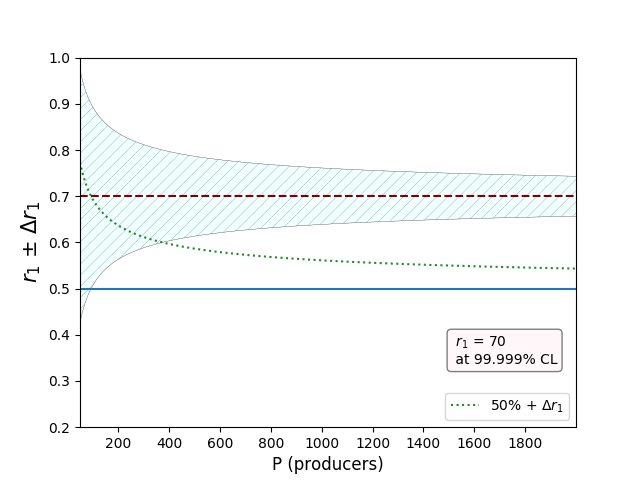
\includegraphics[width=\textwidth]{Figures/r_over_P_at_70}
        \label{fig:rrdeltarb}
    \end{subfigure}
    \begin{subfigure}[b]{0.45\textwidth}
        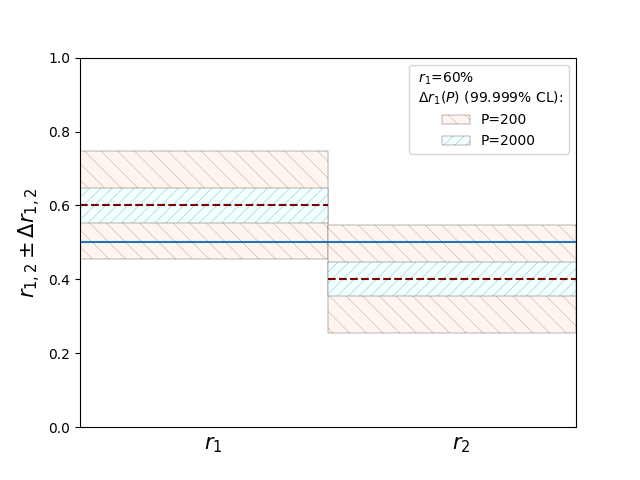
\includegraphics[width=\textwidth]{Figures/r_pm_deltar_at_60}
        \label{fig:rdeltara}
    \end{subfigure}
    \vspace*{-0.2in}
    \caption{Left: $ri \pm \Delta r_i$ $(i=1~or~2)$ as a function of P, the size of the producers pool, when $r_1 = 60\%$. Right: $r \pm \Delta r$ at 99.999\% confidence level, for two values of P (200, 2000) when only two types of hash are collected by a producer, when $r_1 = 70\%$.}
    \label{fig:rdeltar}
\end{figure}


\item $(V_{min}, V_{threshold})$: a producer needs to collect enough individual candidates (at least $V_{min}$) and find a majority (at least $V_{threshold}$) of identical hashes embedded in the candidate to be able to issue a vote. 
$V_{min}$ is typically defined as a fraction of $P$: $V_{min} = f_V P$ with $0 < f_V < 1$. $V_{threshold}$ is defined following the same approach considered for $C_{threshold}$: 
 \begin{equation}
 V_{threshold}(99.999\%) = \left( 0.5 + 4.22\sqrt{\frac{V^{maj}(V_j-V^{maj})}{V_j^3}} \right) \times V_j
 \end{equation}
 
 \item $(U_{min}, U_{threshold}, C_n)$: a producer needs to collect enough individual votes (at least $U_{min}$) and find a majority (at least $U_{threshold}$) of votes with identical hash embedded in these to be able to confidently broadcast the content-based address of the next ledger state update stored on DFS across the network. Two votes are considered identical if they include the same DFS address of a complete ledger state update including the compensation entries that reward the producers for their work. Two complete ledger state updates are therefore identical notably if the lists $\mathcal{L}_{n}(prod)$ used to create the compensation entries are identical. The list $\mathcal{L}_{n}(prod)$ comprises the identifiers of the $C_n$ producers that produced the right ledger state update (without compensation entries) during the construction phase. $C_{n}$ is typically defined as a fraction of $P$: $C_{n} = f_{prod}P$ with $0 < f_{prod} < 1$.
 $U_{min}$ is defined as a fraction of $C_n$: $U_{min} = f_U C_n$ with $0 < f_U < 1$. Indeed $U_{min}$ is a fraction of producers among these that had produced a candidate such that the local ledger update embedded in said candidate corresponding to $\Delta L_n~/|~L_{CE}$. $U_{threshold}$ is defined following the same approach considered for $C_{threshold}$: 
 \begin{equation}
 U_{threshold}(99.999\%) = \left( 0.5 +  4.22\sqrt{\frac{U^{maj}(U_j-U^{maj})}{U_j^3}} \right) \times U_j
 \end{equation}

\end{enumerate}

In summary the probability $\mathcal{P}(x>P/2)$ that $x >P/2$ can be expressed as a function of $P, C_{min} ,C_n, V_{min}, U_{min}$:
%\begin{center}
%$\mathcal{P}(x>P/2) = f(P, C_{min} ,C_n, V_{min}, U_{min})$ 
%\end{center}
\begin{center}
\[
  \mathcal{P}(x>P/2) = f(f_{prod}, f_C, f_V, f_U)\begin{cases}
               f_{prod} = C_n/P, f_C = C_{min}/P\\
               f_V = V_{min}/P, f_{U} = U_{min}/C_n
            \end{cases}
\]
\end{center}
The tests conducted on the gossip protocol implemented on Catalyst suggest that a high percentage of nodes ($95-99\%$) in a large network will successfully collect data from all their peers. Furthermore tests on a smaller networks such as the sub-networks of workers and producers in charge of producing the ledger state update during a ledger cycle gives the percentage of nodes collecting the data from all their peers as close to 100\%. As a result the numbers $(C_{j} ,V_{j})$ of data collected by a producer $P_j$ are naturally expected to be close to $P$ and $U_j$ close to $C_n$. A simulation analysis was done to determine the optimal set of parameters $(C_n, C_{min}, V_{min}, U_{min})$ to ensure a probability $\mathcal{P}(x>P/2)$ greater than 99.999\% for various sizes of the producers pool $P$.
Figure~\ref{fig:tree} displays a \textit{n-ary} tree ($n=4$) illustrating the minimum sets of parameters $(f_{prod}, f_C, f_V, f_U)$ found for a pool of producers made of (a) 200 nodes and (b) 500 nodes when varying the parameters $(f_{prod}, f_C, f_V, f_U)$ between 0.75 and 0.95 with a step of 0.05. We observe that for $P = 200$, when $f_{prod}=80\%$ of producers generate the correct ledger state update, $\mathcal{P}(x>P/2) > 99.999\%$ when all thresholds are set at 80\%. The values represented in the tree branches show how the thresholds naturally decrease as the number $P$ of nodes in the pool of producers increases.


\begin{figure}[H]
\centering
   \begin{subfigure}[b]{0.45\textwidth}
       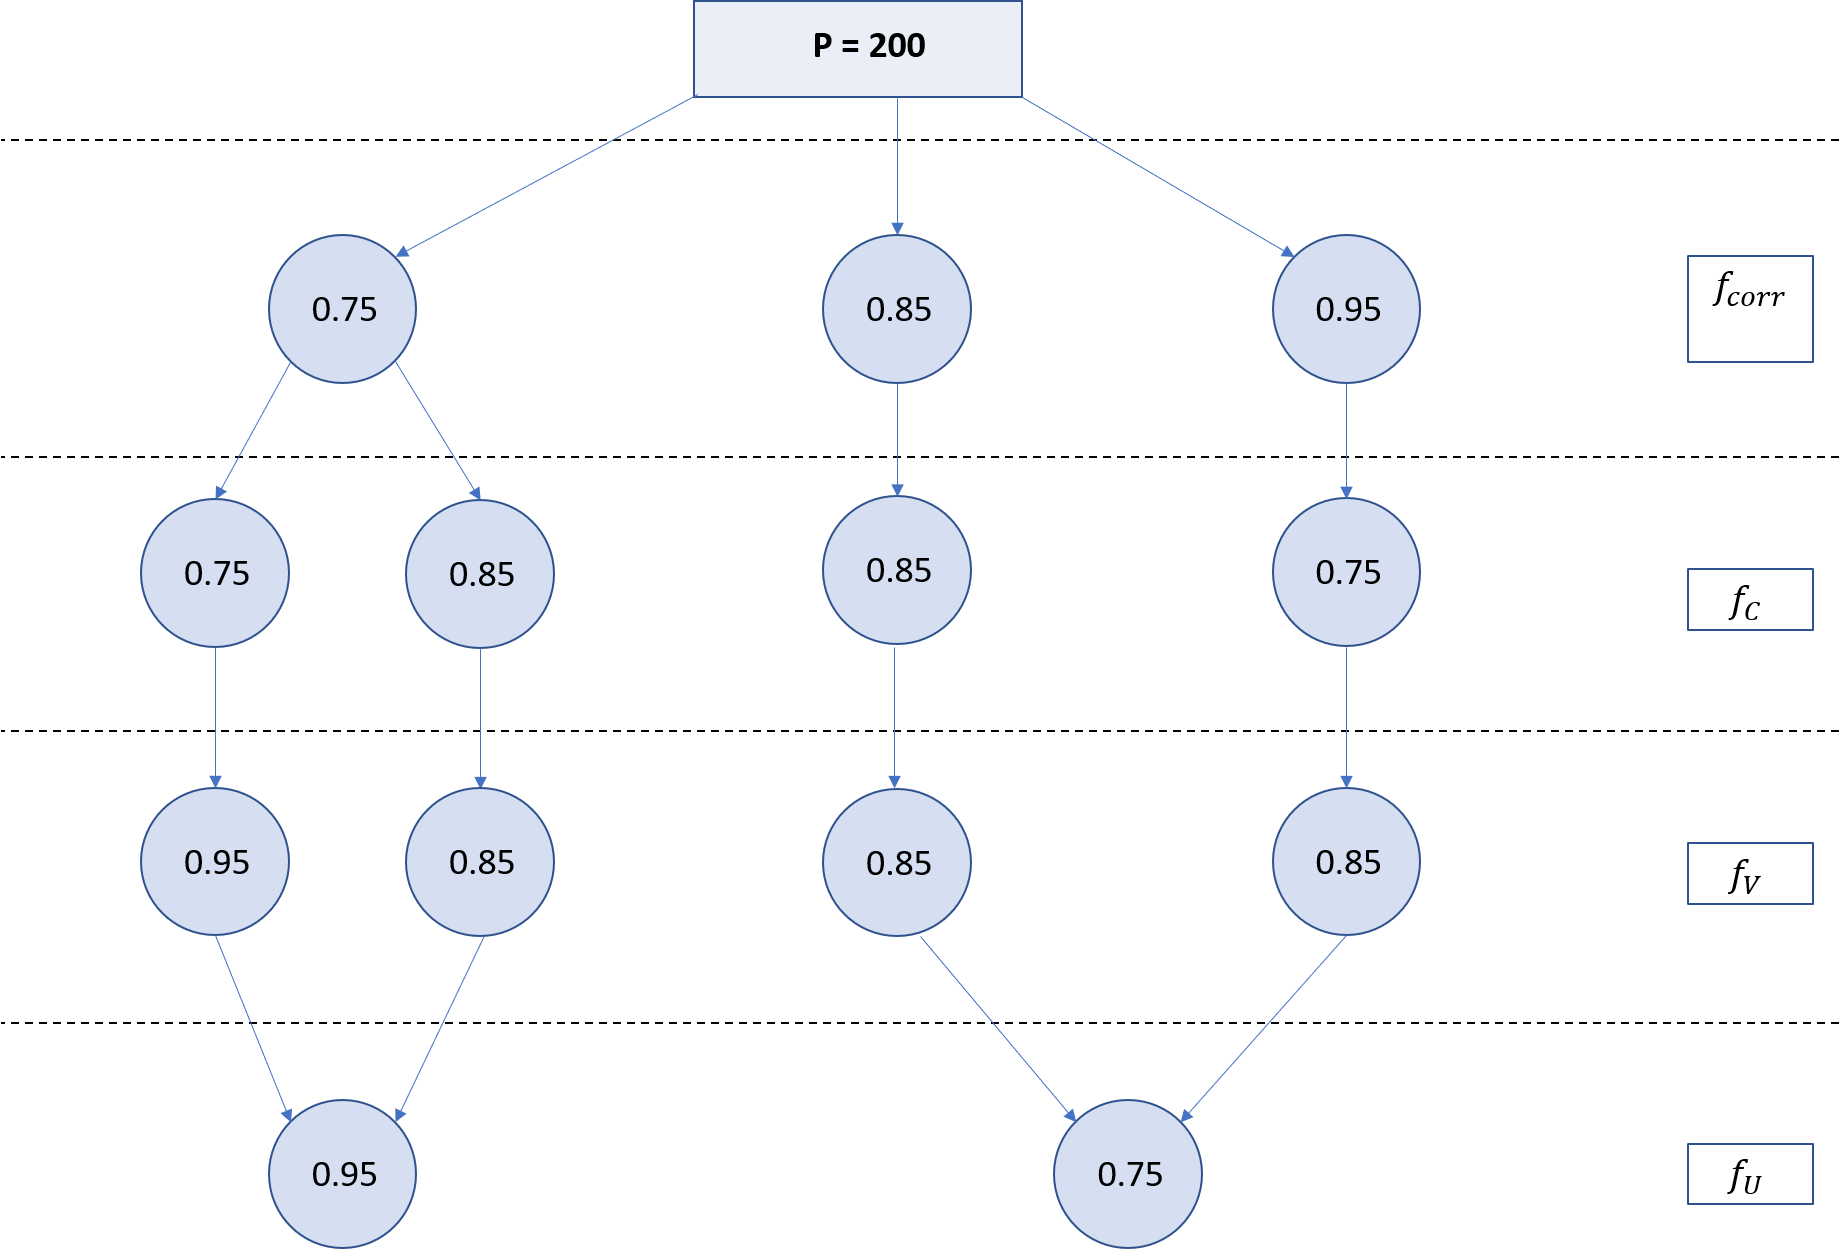
\includegraphics[width=\textwidth]{Figures/tree_P_200}
   \end{subfigure}
   \begin{subfigure}[b]{0.47\textwidth}
       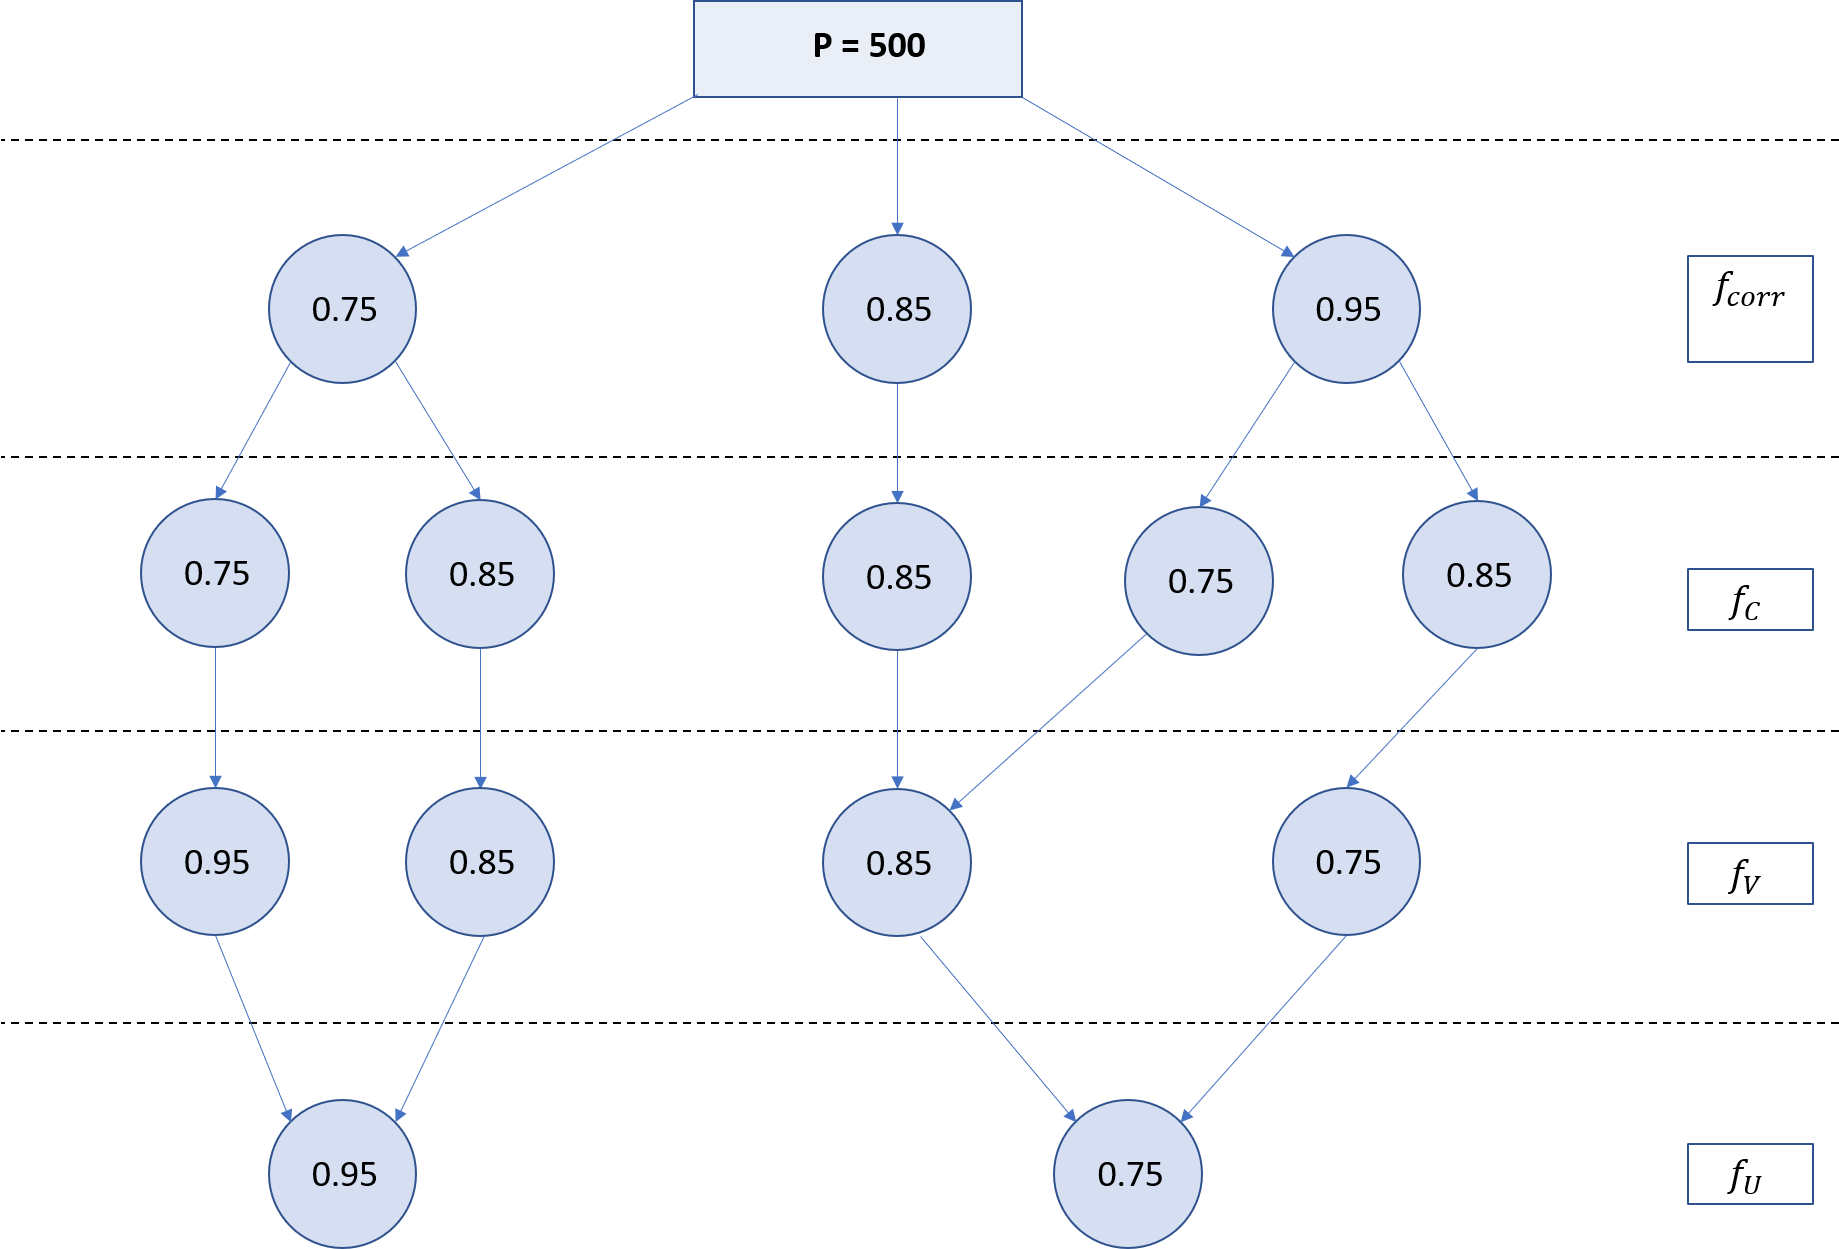
\includegraphics[width=\textwidth]{Figures/tree_P_500}
   \end{subfigure}
   \caption{Minimum sets of parameters $(f_{prod}, f_C, f_V, f_U)$ found for $\mathcal{P}(x>P/2) > 99.999\%$ for P = 200 (left) and P = 500 (right).}
   \label{fig:tree}
\end{figure}

Figure~\ref{fig:treeSum} shows the minimum common threshold found for $(f_C, f_V, f_U)$ as a function $P$ when $f_{prod} = 75\%$ and $f_{prod} = 95\%$. \\


\begin{wrapfigure}{r}{0.4\textwidth}
 \vspace{-1.5cm}
 \begin{center}
   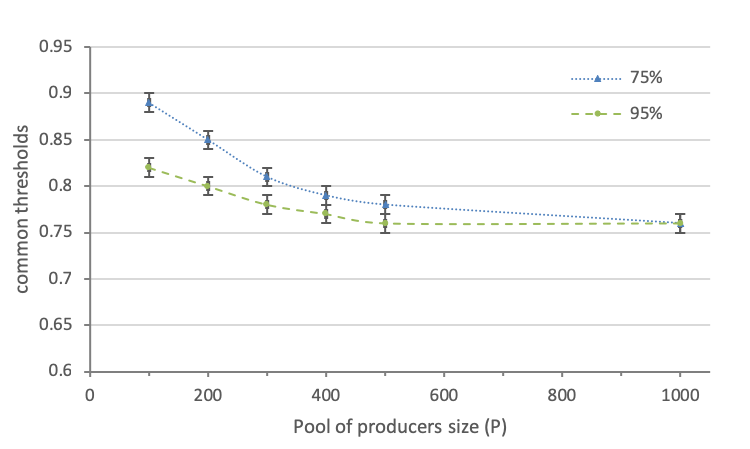
\includegraphics[width=0.4\textwidth]{Figures/tree_summary_p200t1000.png}
 \end{center}
 \vspace{-0.6cm}
  \caption{Minimum common set of parameters $(f_C, f_V, f_U)$ as a function of $P$ when $f_{prod} = 75\%$ (blue) and $f_{prod} = 95\%$ (green).}
   \label{fig:treeSum}
\end{wrapfigure}

At $P=1000$, the two curves converge to a common threshold $f_C=f_V=f_U=76\% \pm 1\%$. When $f_{prod} = 75\%$, we find that in approximately 95\% of the conducted tests, $x=P$, all producers broadcast the same quantity $\mathcal{H}(\Delta L_n)~||~\#(\mathcal{L}_{n}(vote))$. When $P=200$ and $f_{prod} = 75\%$, a higher common threshold $f_C = f_V = f_U = 85\% \pm 1\%$ is found to satisfy $\mathcal{P}(x>P/2) > 99.999\%$ and $x=P$ in roughly 80\% of the tests.\\
\\
The decision regarding the thresholds chosen for generating the ledger state update thus depends on $P$. As explained in section~\ref{Sec:ConSec}, the choice of $P$ as well as that of the worker pool size $N$ also influence the resistance to 51\% attack. Figure~\ref{fig:P} shows that in order to keep the probability of a successful 51\% attack below 1 in a billion when $N=2000$, the size of producers must comprise at least $P=1200$ producers. The simulation conducted in this section shows that when $P \geq 1000$ a common threshold value $f_C = f_V = f_U = 80\%$ ensures that a consensus can be reached at 99.999\% confidence level when $f_{prod}$ $\geq$ 75\% for any $x$ value greater or equal to $P/2$.





\section{Security of the Signature Scheme}\label{Sec:SSS}

\subsection{Rogue Key Attack}

When Schnorr signatures used to generate aggregated signature of a transaction are vulnerable to an attack known as Rogue Key attack. Rogue Key attacks performed by a malicious entity consists of generating an aggregated signature in such a way that they posses the public/private key pair for that signature. In the Schnorr signature scheme, the public key of participants are aggregated and the sum represent the public key associated to the signature. Assume that an honest participant use its public key $Q_a$ in the transaction and a malicious participant possesses $Q_b$. By sending the public key $Q_m = Q_b - Q_a$ to the honest participant, the malicious entity have access to the transaction as they will hold the private key for $Q_b$. This is because when the keys are aggregated i.e. $Q_m + Q_b$ the aggregated signature would be $Q_b$, for which the malicious user holds the private key (the honest user would not). For an aggregated public key, there should be no user that has a private key equivalent as it should be used to create a signature that can be verified that all users in the transaction participated. \\ 	

The aggregation of public keys used in Catalyst which is based on Mu-Sig \cite{musig} signature scheme that is not vulnerable to this form of attack. Mu-Sig is protected from this form of attack as the scheme does not require a user to demonstrate each public key, only the sum of all the public keys. By not verifying individual public keys, a key rogue attack is not possible. Only one public key is needed for the verification (the aggregated key) for which there will not be an equivalent private key.

\subsection{Quantum Attack}

Quantum computers pose a very real threat to the encryption techniques used in blockchains in the medium to long term \cite{agarwal} \cite{kearney}. The threat is through the use of Shor's algorithm. A quantum attacker using Shor's algorithm on a quantum computer can gain an exponential speed-up in solving the discrete logarithmic problem. The assumption of security the discrete logarithmic functions the the primary basis as to which all elliptic curve cryptography is based. This means that even the schema demonstrated here will be vulnerable to attack. The use of aggregated signatures would provide some resistance, however this resistance would be negligible. \\

It must be impressed that this is not an issue for the near term and thereby, these schema are highly secure and efficient currently. The most efficient algorithm for classical computers to solve the discrete logarithm problem is the Pollard's rho\cite{pollard}, this does not run in polynomial time. While Catalyst is not currently resistant to quantum attack, this is a challenge that will be faced by all major distributed ledgers over time. 


%%%%%%%%%%%%%%%%%%%%%%%%%%%%%%%

\chapter*{Conclusion} \label{Cha:Con}
\addcontentsline{toc}{chapter}{Conclusion}

The individual technical components underpinning Distributed Ledger and Blockchain Technologies have existed for decades. As the $1^{st}$ generation blockchain, Bitcoin managed to recombine these previously established elements in a unique fashion so as to instil and enable trust in a trust-less system, thus achieving decentralisation and eliminating the need for a centralised authority. Whilst completely revolutionary at the time, the implementation and expansion of this new approach uncovered limitations and hurdles to both expanded use and ultimately mainstream adoption. $2^{nd}$ generation DLTs and blockchains built and improved upon this original foundation but fall short of resolving all associated issues. \\
 
Atlas City has developed a distributed operating system, Catalyst, to solve the issues of previous DLTs and blockchains, improving upon those which came before, resolving such challenges and enabling an equitable and proportionate compensation to participants on the network. Catalyst was designed around the notion that a democratic and ethical network can exist which is secure, decentralised, scalable and private.  \\
 
Catalyst code base does not fork from a previously existing projects and includes original and innovating work, including a new collaborative and environment-friendly consensus-based protocol, the possibility to process both confidential and non-confidential transactions as well as smart contracts, an efficient peer-to-peer communication layer and a multi-level data architecture for a lean ledger database storing a variety of data.\\
 
This paper gives an overview of Catalyst core protocol. Another paper, currently under preparation, presents network performances measurement. 







%NEEDS UPDATING AND REORDERING
\begin{thebibliography} {unsrt}
\bibitem{BFT} G. Konstantopoulos, 2017. \url{https://medium.com/loom-network/understanding-blockchain-fundamentals-part-1-byzantine-fault-tolerance-245f46fe8419}
\bibitem{bc24} \url{https://www.blockchain.com/pools?timespan=24hours} 
\bibitem{pool_cent} \url{https://www.buybitcoinworldwide.com/mining/pools}
\bibitem{PoSr} C. Lacina, 2015. \url{https://cointelegraph.com/news/the-inevitable-failure-of-proof-of-stake-blockchains-and-why-a-new-algorithm-is-needed}
\bibitem{schnorr} G. Maxwell \textit{et al.} {\em Simple Schnorr Multi-Signatures with Applications to Bitcoin} 20 May 2018 Last Accessed 08/02/19: \url{https://pdfs.semanticscholar.org/a4da/14a4329d7bf28e2ecbf9a3e42bf1faba523e.pdf?_ga=2.193608301.1119480105.1549621665-1692475185.1549621665} 
\bibitem{agarwal} D. Aggarwal, 2018. {\em Quantum attacks on Bitcoin, and how to protect against them. Quantum Physics}. arXiv:1710.10377
\bibitem{pollard} A. Koundinya, 2013. {\em Performance Analysis of Parallel Pollard's Rho Factoring Algorithm}. International Journal of Computer Science \& Information Technology (IJCSIT)
\bibitem{musig} G. Maxwell, 2018. {\em Simple Schnorr Multi-Signatures with Applications to Bitcoin}. \url{https://eprint.iacr.org/2018/068}
\bibitem{confidential} G. Maxwell, 2015 {\em Confidential Transactions}. \url{https://people.xiph.org/~greg/confidential_values.txt}
\bibitem{bulletproof} B. B\''{u}nz \textit{et al.}, 2019. {\em Bulletproofs:  Short Proofs for Confidential Transactions and More}.  \url{https://eprint.iacr.org/2017/1066.pdf}
\bibitem{monero} Monero, 2014-2019. {\em Monero: the secure, private, untraceable cryptocurrency}  \url{https://github.com/monero-project/monero/tree/bc208be63d880871f4f1d6b51a7b35abd5e9b8f0}
\bibitem{NSA} D. J. Bernstein and T. Lange, 2016.  {\em Failures in NIST's ECC standards}. \url{https://cr.yp.to/newelliptic/nistecc-20160106.pdf}
\bibitem{ed25519} D. J. Bernstein, 2017. {\em Ed25519: high-speed high-security signatures}. \url{https://ed25519.cr.yp.to/}
\bibitem{blake} \url{https://coinguides.org/blake2b/}
\bibitem{electric} \url{https://digiconomist.net/ethereum-energy-consumption}
\bibitem{swis} B. Gehring, 2018. {\em Swiss Payment Monitor 2018}, p18. \url{swisspaymentmonitor.ch}
\bibitem{EthTxpD} \url{https://etherscan.io/chart}, 21/05/2019
\bibitem{BitTxpD} \url{https://www.blockchain.com/en/charts}, 21/05/2019
\bibitem{kearney} J. J. Kearney and C. A. P\'erez-Delgado, 2019. {\em Blockchain Technologies Vulnerability to Quantum Attacks}

\end{thebibliography}


\end{document}